\documentclass[11pt,a4paper,toc=bibliography]{scrartcl}
%Packages%
\usepackage[utf8]{inputenc}
\usepackage[ngerman]{babel}
\usepackage[T1]{fontenc}
\usepackage{graphicx}
\usepackage{amsmath}
\usepackage{amsfonts}
\usepackage{amssymb}
\usepackage{amsthm}
\usepackage{mathtools}
\usepackage{faktor}
\usepackage{lmodern}
\usepackage{longtable}
\usepackage[plainpages=false]{hyperref}
\usepackage{theoremref}
\usepackage{tikz-cd}
\usepackage{standalone}
\usepackage[automark]{scrpage2}
\usepackage[german]{nomencl}
\RequirePackage{
ifthen}
\ihead{\headmark}
\chead{}
\pagestyle{scrheadings}

\addtokomafont{section}{\huge}
\addtokomafont{subsection}{\Large}
\addtokomafont{subsubsection}{\large}



\oddsidemargin=0.in
\topmargin=-1.5cm
\textheight=23cm
\textwidth=16cm
\title{{\Huge Bachelorarbeit} \\[18pt] Ein Endlichkeitssatz für die 1. Kohomologiegruppe von kompakten Riemannschen Flächen \\[18pt]}
\author{Aurelio Marafioti}

%Theoreme%
\newtheoremstyle{thm}{20pt}{20pt}{\itshape}{}{\bfseries}{.}{1em}{}
\newtheoremstyle{def}{20pt}{20pt}{}{}{\bfseries}{.}{1em}{}
\theoremstyle{thm}
\newtheorem{satz}{Satz}[section]
\newtheorem{lemma}{Lemma}[section]
\newtheorem{koro}{Korollar}[section]
\theoremstyle{def}
\newtheorem{defi}{Definition}[section]
\newtheorem{bsp}{Beispiel}[section]
\theoremstyle{remark}
\newtheorem*{bem}{Bemerkung}

%Operatoren%
\DeclareMathOperator{\id}{id}
\DeclareMathOperator{\Ima}{Im}
\DeclareMathOperator{\ord}{ord}




%Befehle%
\newcommand*{\norm}[1]{\left\lVert#1\right\rVert} %Eine Norm%
\newcommand*\dif{\mathop{}\!\mathrm{d}}\newcommand{\einschraenkung}{\,\rule[-5pt]{0.4pt}{12pt}\,{}} %Ein d für dx%

%erneuerte Befehle%
\renewcommand{\labelenumi}{(\roman{enumi})} %Aufzählungen mit römischen Schriftzeihen%
\renewcommand{\theequation}{\thesubsection.\arabic{equation}} %Equations und figures mit arabaischen Zahlen nummerieren%
\renewcommand{\thefigure}{\thesubsection.\arabic{equation}}
\renewcommand{\nomgroup}[1]{%
\ifthenelse{\equal{#1}{G}}{\item[\large\textbf{Garben und Funktionenräume}]}{%
\ifthenelse{\equal{#1}{A}}{\item[\large\textbf{Generelle Notation}]}{%
\ifthenelse{\equal{#1}{K}}{\item[\large\textbf{Kohomologietheorie}]}{
\ifthenelse{\equal{#1}{O}}{\item[\large\textbf{Sonstiges}]}}}}
}
\renewcommand{\pagedeclaration}[1]{S.#1}


%Einstellungen für Paragraphen%
\setlength{\topsep}{0pt}
\setlength{\partopsep}{15pt plus 1pt minus 1pt}
\setlength{\parskip}{10pt}
\setlength{\parindent}{0pt}

\date{\today}

\makenomenclature

\begin{document}
\documentclass[10pt,a4paper]{article}
\usepackage[utf8]{inputenc}
\usepackage[german]{babel}
\usepackage{amsmath}
\usepackage{amsfonts}
\usepackage{amssymb}
\usepackage{graphicx}
\usepackage[top=1cm,bottom=1cm]{geometry}

\begin{document}
	

		\begin{center} 
			
\includegraphics[scale=0.4]{./Dateien/UniKoelnLogo.jpeg}
			\vspace*{2cm} 
			
			
			\large 
			Bachelorarbeit
			\vspace*{2cm}
			
			{\huge \textbf{Der Endlichkeitssatz für $H^1(X,\mathcal{O})$ auf kompakten Riemannschen Flächen}}
			\vspace*{1cm}
			
			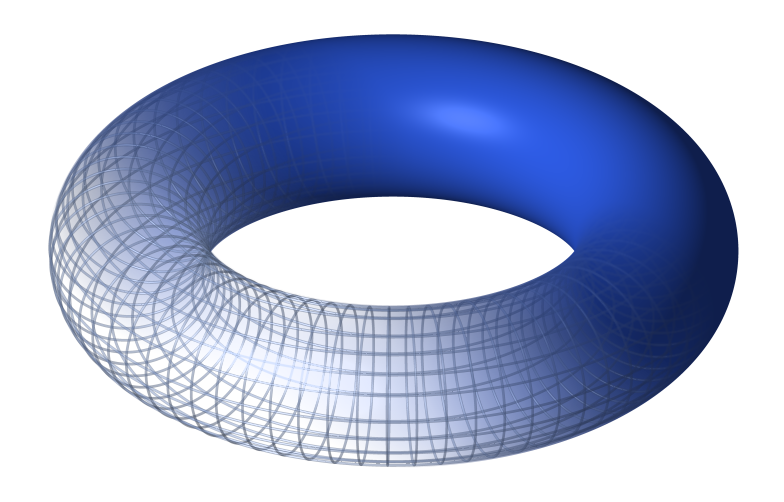
\includegraphics[scale=0.2
			]{./Dateien/Torus.png}
			\vspace{2.5cm}
			
			Aurelio Marafioti
			
			7306409
			\vspace*{1cm}
			
			\today
			\vspace*{2cm}
			
			
			Betreuung: Prof. Dr. George Marinescu \\
			Mathematisches Institut \\
			Universität zu Köln
		\end{center}

\end{document}
\pagenumbering{Alph}
% Erzeugung des Deckblatt


\thispagestyle{empty}

\newpage

\tableofcontents

\thispagestyle{empty}


\newpage
\pagenumbering{arabic}
\section{Einleitung}
\newpage




\nomenclature[Aa]{$\mathbb{N}$}{Menge der natürliche Zahlen}
\nomenclature[Ab]{$\mathbb{Z}$}{Ring der ganzen Zahlen}
\nomenclature[Ac]{$\mathbb{R}$}{Körper der reellen Zahlen}
\nomenclature[Ad]{$\mathbb{C}$}{Körper der komplexen Zahlen}
\nomenclature[Ae]{$\mathbb{C}^*$}{$=\{z\in\mathbb{C};~z\neq 0\}$}
\nomenclature[Af]{$\mathbb{P}_1$}{$=\mathbb{C}\cup \{\infty\},$ die Riemannsche Zahlenkugel}

%SECTION:EINFÜHRUNG%

\section{Einführung}
\phantom{\cite{algCur}\cite{algTop}}
%subsection:Einführung in die Garbentheorie%

\subsection{Einführung in die Garbentheorie}
Hier wird zunächst eine Einführung in die Theorie der Garben gegeben, welche sich mithilfe der Garbenkohomologie als sehr nützliches Werkzeug für die Untersuchung der Riemannschen Flächen erweisen wird. 	Unter den ersten Definitionen lassen sich motivierende Beispiele finden.


\begin{defi}[Prägarbe]\thlabel{defi:praegarbe}
Sei $X$ ein topologischer Raum und $\mathcal{T}$ die Topologie auf X. Eine \emph{Prägarbe} abelscher Gruppen ist ein Paar $(\mathcal{F},\rho)$, bestehend aus:

\begin{itemize}
\item
Einer Familie $\mathcal{F}=(\mathcal{F}(U))_{U\in \mathcal{T}}$ abelscher Gruppen
\item
Einer Familie $\rho=(\rho^U_V)_{U,V\in\mathcal{T}, V \subset
U}$ von Gruppenhomomorphismen $\rho^U_V:\mathcal{F}(U)\rightarrow \mathcal{F}(V)$.
\end{itemize}
Diese sollen auf natürliche Weise zusammenpassen, das bedeutet:
\begin{enumerate}
\item $
\rho^U_U =\textstyle{ \id_{\mathcal{F}(U)}}
$
\item $\rho_V^W\circ \rho_V^U=\rho_W^U$
\end{enumerate}



für alle $W\subset V\subset U$ offen in $X$.
Die Elemente in $\mathcal{F}(U)$ für $U\subset X$ offen heißen \emph{(lokale) Schnitte} und die Elemente in $\mathcal{F}(X)$ heißen \emph{globale Schnitte}.
Wir schreiben für einen Schnitt $f\in\mathcal{F}(U)$ auch $p^U_V(f)=f \mid V$ und nennen die $p^U_V$ \emph{Einschränkungshomomorphismen}. Außerdem schreibt man oft nur $\mathcal{F}$ statt $(\mathcal{F},p)$, wenn die Einschränkungshomomorphismen in natürlicher Weise gegeben sind (siehe dazu die Beispiele).
\end{defi}

\begin{defi}[Garbe]\thlabel{defi:garbe}
Sei X ein topologischer Raum und $(\mathcal{F},p)$ eine Prägarbe abelscher Gruppen auf $X$.
Falls nun für jede offene Menge $U\subset X$ und jede Familie von offenen Mengen $U_i\subset U$ mit $U = \bigcup_{i\in I}$ gilt:
\renewcommand{\labelenumi}{(\roman{enumi})}
\begin{enumerate}
\item
Für $f,g\in \mathcal{F}(U)$ mit $f\mid U_i = g\mid U_i$ gilt $f=g$,
\item
Gegeben $f_i\in U_i$ mit 
$f_i\mid U_i\cap U_j = f_j\mid U_i\cap U_j$ für alle $i,j\in I$,
so gibt es ein $f\in \mathcal{F}(U)$, sodass $f\mid U_i= f_i$ für alle $i\in I$,
\end{enumerate}
dann heißt $(\mathcal{F},p)$ \emph{Garbe}. Diese Eigenschaften nennt man \emph{Garbenaxiome}.
\end{defi}
\begin{bem}
Analog dazu lassen sich Prägarben, sowie Garben auch auf Vektorräumen,Ringen und weiteren algebraischen Objekten definieren. 
\end{bem}

\begin{bsp}

\begin{enumerate}
\item
Für einen topologischen Raum $X$ und $U\subset X$ offen sei $\mathcal{C}(U)$ der Vektorraum aller stetigen Funktionen $f:U\rightarrow \mathbb{C}$.
Für $V\subset U $ offen sei $p^U_V: \mathcal{C}(U)\rightarrow \mathcal{C}(V)$ der übliche Einschränkungshomomorphismus. Dann ist $\mathcal C = (\mathcal C,p)$ eine Garbe von Vektorräumen, genannt Garbe der stetigen Funktionen auf X.
\item
Seien $X$ eine Riemannsche Fläche und und $\mathcal{O}(U)$ für $U\subset X$ offen die holomorphen Funktionen 
$f:U\rightarrow \mathbb{C}$. Mit dem üblichen Einschränkungshomomorphismus bildet auch $\mathcal{O}$ eine Garbe von Vektorräumen, genannt Garbe der holomorphen Funktionen.
Analog bildet $\mathcal{M}$ die Garbe der meromorphen Funktionen auf $X$ und $\mathcal{E}$ die der stetigen.
\item  Sei $\mathcal{B}(U) $  für $U\subset \mathbb{C}$  offen die Menge aller beschränkten, holomorphen Funktionen $f:U\rightarrow \mathbb{C}$. Zusammen mit den natürlichen Einschränkungshomomorphismen ist $ \mathcal{B}$ eine Prägarbe. Seien $U_i=\{ z\in\mathbb{C};|z|<i\}$ für $i\in\mathbb{N}$,  dann bilden diese Mengen eine offene Überdeckung von $\mathbb{C}$.  Betrachten wir nun die Funktionen $f_i (z)\in \mathcal{B}(U_i)$,  dann gilt $f_i\mid U_i\cap U_j= f_j\mid U_i\cap U_j$ für alle $i,j\in \mathbb{N}$, aber es gibt keinen globalen Schnitt $f\in\mathcal{B}(\mathbb{C})$ mit $f\mid U_i = f_i$, denn diese Funktion wäre unbeschränkt. Damit wird das zweite Garbenaxiom nicht erfüllt und $\mathcal{B}$ ist keine Garbe.
\nomenclature[Gb]{$\mathcal{O}$}{Garbe der holomorphen Funktionen, \nomrefpage}
\nomenclature[Ga]{$\mathcal{E}$}{Garbe der differenzierbaren Funktionen, \nomrefpage}
\nomenclature[Gc]{$\mathcal{M}$}{Garbe der meromorphen Funktionen, \nomrefpage}
\end{enumerate}


\end{bsp}

Als nächstes interessiert uns, wie die Elemente der $\mathcal{F}(U)$ in der Nähe eines Punktes $a\in X$ aussehen. Wir betrachten dazu die disjunkte Vereinigung
\[
\dot{\bigcup_{U\in \mathcal{T},a\in U}} \mathcal{F}(U).
\]

\begin{defi}[Halm,Keim]\thlabel{defi:halm}
Sei $\mathcal{F}$ eine Garbe auf dem topologischen Raum ($X,\mathcal{T}$). Zwei Elemente $f\in\mathcal{F}(U)$ und $g\in \mathcal{F}(V)$ für $U,V\subset X$ offen und $a\in U\cap V$ heißen äquivalent,
\[
f\sim_a g,
\]
genau dann, wenn es eine offene Menge $W\subset X$ mit $a\in W\subset U\cap V$ gibt mit
\[
f\mid W = g\mid W.
\]
In anderen Worten sind diese in der Nähe von $a$ gleich. Dann ist die Menge (abelsche Gruppe, Vektorraum, etc.)
\[
\mathcal{F}_a \coloneqq \left( \dot{\bigcup_{U\ni a}} \mathcal{F}(U) \right) /\sim_a
\]
der \emph{Halm} der Garbe $\mathcal{F}$ in $a$. Die Elemente eines Halms, also Äquivalenzklassen, heißen $Keime$.
\end{defi}
\nomenclature[Gd]{$\mathcal{F}_a$}{Halm der Garbe $\mathcal{F}$ im Punkt $a$, \nomrefpage}
\begin{bsp}
Für die Garbe $\mathcal{O}$ der holomorphen Funktionen auf $\mathbb{C}$ ist ein Element von $\mathcal{O}_a$ repräsentiert durch eine holomorphe Funktion in einer offenen Umgebung von $a$. Also kann man diese mit ihrer Taylorentwicklung als
\[
\sum_{i=0}^{\infty} c_i(z-a)^i
\]
schreiben. Dann repräsentieren zwei Funktionen den selben Keim genau dann, wenn sie die selbe Taylorentwicklung besitzen, also ist 
\[
\mathcal{O}_a \cong \mathbb{C}\{ z-a \},
\]
wobei letzteres der Ring der konvergenten Potenzreihen um $(z-a)$ mit komplexen Koeffizienten ist.
\end{bsp}

Man kann für Garben nun auch Homomorphismen definieren und damit den Begriff der exakten Sequenz.

\begin{defi}[Garbenhomomorphismus]\thlabel{defi:garbenhomomorhpismus}
Seien $(\mathcal{F},\rho),(\mathcal{G},\rho')$ Garben abelscher Gruppen über dem topologischen Raum $X$. 
Als \emph{Garbenhomomorpismus} bezeichnen wir eine Familie von Gruppenhomomorphismen 
\[
\alpha_U :\mathcal{F}(U)\rightarrow \mathcal{F}(V)
\]
für $U\subset X$ offen, sodass diese kompatibel mit den jeweiligen Einschränkungsabbildungen sind. 
Damit ist gemeint, dass das Diagramm
\begin{center}
\begin{tikzcd}
\mathcal{F}(U) \arrow{d}[swap]{\rho^U_V} \arrow{r}{\alpha_U}
& \mathcal{G}(U)\arrow{d}{{\rho'}^U_V} \\
\mathcal{F}(V) \arrow{r}{\alpha_V} &\mathcal{G(V)} \\ 
\end{tikzcd}
\end{center}
für $U\subset V$ offen kommutiert. 
Sind alle $\alpha_u$ Gruppenisomorphismen, so heißt $\alpha$ \emph{Garbenisomorphismus}. 
Analog kann man die Definition für Ringe und Vektorräume formulieren.
\end{defi}

\begin{defi}[Exakte Sequenz]\thlabel{defi:exakte sequenz}
Ein Garbenhomomorphismus $\alpha : \mathcal{F}\rightarrow \mathcal{G}$ induziert für alle $x\in X$ einen Homomorphismus der Halme 
\[
\alpha_x : \mathcal{F}_x \rightarrow \mathcal{G}_x.
\]
Wir nennen dann eine Sequenz
\begin{center}
\begin{tikzcd}[row sep =small, column sep = small]
\mathcal{F}\rar{\alpha}&\mathcal{G}\rar{\beta}&\mathcal{H}
\end{tikzcd}
\end{center}
von Garbenhomomorphismen \emph{exakt}, falls die Sequenz
\begin{center}
\begin{tikzcd}[row sep =small, column sep = small]
\mathcal{F}_x\rar{\alpha_x}&\mathcal{G}_x\rar{\beta_x}& \mathcal{H}
\end{tikzcd}
\end{center}
exakt ist , also $\ker \beta_x =\Ima \alpha_x$.
Analog nennen wir die Sequenz
\begin{center}
\begin{tikzcd}[row sep =small, column sep = small]
\mathcal{F}_1\ar{r}{\alpha_1} & \mathcal{F}_2\ar{r}{\alpha_2}&\ldots \ar{r}{\alpha_{n-2}}&\mathcal{F}_{n-1}\ar{r}{\alpha_{n-1}} & \mathcal{F}_n\\
\end{tikzcd}
\end{center}
\emph{exakt}, falls für $1\leq k\leq n-2$ die Sequenzen
\begin{center}
\begin{tikzcd}[row sep =small, column sep = small]
\mathcal{F}_k\ar{r}{\alpha_k} &\mathcal{F}_{k+1}\ar{r}{\alpha_{k+1}} &\mathcal{F}_{k+2}
\end{tikzcd}
\end{center}
exakt sind.
Ein Garben\emph{monomorphismus} ist ein Garbenhomomorphismus, sodass 
\begin{center}
\begin{tikzcd}[row sep =small, column sep = small]
0\rar &\mathcal{F}\rar{\alpha} &\mathcal{G}
\end{tikzcd}
\end{center}
exakt ist und ein Garben\emph{epimorphismus} ein solcher, sodass
\begin{center}
\begin{tikzcd}[row sep =small, column sep = small]
\mathcal{F}\rar{\alpha} &\mathcal{G}\rar{} & 0
\end{tikzcd}
\end{center}
exakt ist.
\end{defi}

%subsection:Garbenkohomologie%
%subsection:Garbenkohomologie%
\subsection{Garbenkohomologie}
In diesem Abschnitt werden wir nun die Kohomologie von Garben erläutern, um die erste Kohomologiegruppe $H^1(X,\mathcal{F})$ für eine Riemannschen Fläche $X$ und eine Garbe $\mathcal{F}$ zu definieren.
\nomenclature[Kb]{$Z^1(\mathfrak{U},\mathcal{F})$}{erste Kozykelgruppe, \nomrefpage}
\nomenclature[Kc]{$B^1(\mathfrak{U},\mathcal{F})$}{erste Korandgruppe, \nomrefpage}
\nomenclature[Kd]{$\delta$}{Korandoperatoren, \nomrefpage}
\nomenclature[Ka]{$C^q(\mathfrak{U},\mathcal{F})$}{$q$-te Kozykelgruppe\nomrefpage}

\begin{defi}[Kokettengruppe]\thlabel{defi:kokettengruppe}
Sei $X$ ein topologischer Raum und $\mathcal{F}$ eine Garbe abelscher Gruppen auf $X$. Außerdem sei eine offene Überdeckung $\mathfrak{U}= (U_i)_{i\in I}$ von $X$ gegeben.
Definiere für $q =0,1,2,...$ die \emph{q-te Kokettengruppe} von $\mathcal(F)$ bezüglich der Überdeckung $\mathfrak{U}$ als 
\[
C^q(\mathfrak{U},\mathcal{F}) \coloneqq \prod_{(i_0,...,i_q)\in I^{q+1}} \mathcal{F}(U_{i_0}\cap \cdots\cap U_{i_q}). 
\]
Die Elemente von $C^q(\mathfrak{U},\mathcal{F})$ heißen \emph{q-Koketten} und sind Familien
$
(f_{i_0,...,i_q})_{i_0,...,i_q\in I}, 
$
sodass
\[
 f_{i_0,...,i_q}\in\mathcal{F}(U_{i_0}\cap \ldots \cap U_{i_q})
\]
für alle $(i_0,\ldots,i_q)\in I^{q+1}$.
Die Addition zweier Koketten sei komponentenweise definiert.
\end{defi}

\begin{defi}[Kozykel, Koränder]\thlabel{defi:kozykel}
Seien die \emph{Korandoperatoren}
\begin{align*}
&\delta : C^0(\mathfrak{U},\mathcal{F})\rightarrow C^1(\mathfrak{U},\mathcal{F})\\
&\delta:C^1(\mathfrak{U}, \mathcal{F}) \rightarrow C^2(\mathfrak{U},\mathcal{F})
\end{align*}
wie folgt definiert:
\begin{enumerate}
\item
Für $(f_i)_{i\in I}$ sei $\delta ((f_i)) = (g_{i,j})$, wobei
\[
g_{i,j} = f_j-f_i \in \mathcal{F}(U_i\cap U_j)
\]
Die Komponenten auf der rechten Seite werden zunächst auf $U_i\cap U_j$ eingeschränkt und dann subtrahiert.
\item
Für $(f_{i,j})_{i,j\in I}\in C^1(\mathfrak{U}, \mathcal{F})$ sei $\delta ((f_{i,j})) = (g_{i,j,k})$, wobei
\[
g_{i,j,k}\coloneqq f_{j,k}-f_{i,k}+f_{i,j} \in \mathcal{F}(U_i\cap U_j \cap U_k).
\]
Wieder werden hier die Komponenten auf der rechten Seite zunächst eingeschränkt auf $U_i\cap U_j\cap U_k$.
\end{enumerate}
\vspace{0.5cm}
Wegen der komponentenweisen Addition bilden die Korandoperatoren Gruppenhomomorphismen. Seien nun
\begin{align*}
&Z^1(\mathfrak{U}, \mathcal{F}) \coloneqq \ker {(\delta:C^1(\mathfrak{U}, \mathcal{F}) \overset{\delta}{\rightarrow} C^2(\mathfrak{U},\mathcal{F}))}, \\
&B^1(\mathfrak{U}, \mathcal{F}) \coloneqq \Ima {(\delta:C^0(\mathfrak{U}, \mathcal{F}) \overset{\delta}{\rightarrow} C^1(\mathfrak{U},\mathcal{F}))}.
\end{align*}
Die Elemente aus $Z^1(\mathfrak{U}, \mathcal{F})$ heißen \emph{(1-)Kozykel} und die aus $B^1(\mathfrak{U}, \mathcal{F})$ \emph{(1-)Koränder}.
\end{defi}
Folglich ist eine 1-Kokette $(f_{i,j})\in C^1(\mathfrak{U},\mathcal{F})$ genau dann ein Kozykel,
wenn
\[
f_{i_k} = f_{i,j}+f_{j,k} \text{ auf } U_i\cap U_j\cap U_k  
\]
für alle $i,j,k\in I$ gilt.
 Man nennt dies die \emph{Kozykelrelation}. Es folgt, dass $f_{i,i} = 0$ und $f_{i,j} = -f_{j,i}$ gilt, wenn man $i=j=k$ bzw. für letzteres $k=i$ setzt. 

Außerdem ist jeder Korand demnach ein Kozykel und wird auch \emph{zerfallender Kozykel} genannt.
Ein 1-Kozykel $(f_{i,j})\in Z^1(\mathfrak{U}, \mathcal{F})$ zerfällt genau dann, wenn eine 0-Kokette $ (g_i) \in C^0(\mathfrak{U}, \mathcal{F})$ existiert, sodass 
\[
f_{i,j} = g_j-g_i \text{ auf } U_i\cap U_j
\]
für alle $i,j\in I$.

\nomenclature[Ke]{$H^1(\mathfrak{U},\mathcal{F})$}{erste Kohomologiegruppe bezüglich der Überdeckung \mathfrak{U}, \nomrefpage}

\begin{defi}[1.Kohomologiegruppe bzgl. der Überdeckung $\mathfrak{U}$]
Die Quotientengruppe 
\[
H^1(\mathfrak{U},\mathcal{F})\coloneqq  {Z^1(\mathfrak{U}, \mathcal{F})}/{B^1(\mathfrak{U}, \mathcal{F})} 
\]
heißt \emph{1. Kohomologiegruppe} mit Koeffizienten in $\mathcal{F}$ bezüglich der Überdeckung $\mathfrak{U}$.
Die Elemente heißen \emph{Kohomologieklassen} und zwei Kozykel in der selben Kohomologieklasse heißen \emph{kohomolog}.
\end{defi}
Zwei Kozykel sind also genau dann kohomolog, wenn ihre Differenz ein Korand ist bzw. wenn sie zerfällt.
Diese Definition hängt noch von der ausgewählten Überdeckung ab, wir wollen sie aber nur noch von der Riemannschen Fläche $X$ abhängig machen. Die Idee hinter den folgenden Definitionen ist, eine immer feinere Überdeckung zu wählen, um schließlich die Kohomologiegruppe zu erhalten.
\nomenclature[Ai]{$\mathfrak{V}<\mathfrak{V}$}{feinere Übderdeckung\nomrefpage}
\nomenclature[Kf]{$\tau^{\mathfrak{U}}_{\mathfrak{V}}$}{\nomrefpage}
\begin{defi}[feinere Überdeckung]\thlabel{defi:feiner}
Eine offene Überdeckung $\mathfrak{V}=(V_k)_{k\in K}$ wird \emph{feiner} als eine offene Überdeckung $\mathfrak{U}=(U_i)_{i\in I}$ für zwei beliebige Indexmengen $I$ und $K$ genannt, $\mathfrak{V}<\mathfrak{U}$, falls eine Abbildung 
\begin{align*}
\tau: & K\rightarrow I,\\
	  & k\mapsto \tau k
\end{align*}
mit
\[
V_{k}\subset U_{\tau k}
\]
existiert, genannt \emph{Verfeinerungsabbildung}. Das bedeutet, dass jedes $V_k$ in mindestens einem $U_i$ komplett enthalten ist.

Diese Abbildung induziert eine Abbildung
\begin{align*}
\tau_{\mathfrak{V}}^{\mathfrak{U}}:& Z^1(\mathfrak{U},\mathcal{F})\rightarrow Z^1(\mathfrak{V},\mathcal{F})\\
&(f_{i,j})\mapsto (g_{k,l}),
\end{align*}
wobei 
\[
g_{k,l} \coloneqq  f_{\tau k,\tau l}\mid V_k\cap V_l\text{ für } k,l\in K.
\]

Folglich bleibt das Zerfallen eines Kozykels unter der Abbildung erhalten, das es wird auch eine Abbildung 
\[
\tau_{\mathfrak{V}}^{\mathfrak{U}}:H^1(\mathfrak{U},\mathcal{O})\rightarrow H^1(\mathfrak{V},\mathcal{O})
\]
induziert.
\end{defi}
Es muss noch folgendes gezeigt werden, damit diese Abbildung wohldefiniert ist und wir sie zur Definition der Kohomologiegruppe nutzen können:
\begin{lemma}\thlabel{lemma:verfeinerungsabbildung}
Die oben genannte induzierte Abbildung zwischen Kohomologiegruppen  hängt nicht von der Wahl der Verfeinerungsabbildung ab und ist injektiv.
\end{lemma}
\begin{proof}
Zunächst wird der erste Teil gezeigt. Sei also eine weitere Verfeinerungsabbildung  $\tilde{\tau}:K\rightarrow I, (f_{i,j})\mapsto (\tilde{g}_{k,l})$ gegeben. Dann ist $V_K\subset U_{\tau k}\cap U_{\tilde{\tau}k}$ für alle $k\in K$, folglich ergibt die Definition 
\[
h_k\coloneqq f_{\tau k,\tilde{\tau} k}\mid V_k\in \mathcal{F}(V_k)
\]
Sinn. Schließlich gilt auf $V_k\cap V_l$
\begin{align*}
g_{k,l}-\tilde{g}_{k,l} & =f_{\tau k,\tau l}-f_{\tilde{\tau}k,\tilde{\tau}l}\\
& =f_{\tau k,\tau l} +f_{\tau l,\tilde{\tau}k}-f_{\tau l,\tilde{\tau}k}-f_{\tilde{
\tau} k,\tilde{\tau}l}\\ 
						& = f_{\tau k, \tilde{\tau}k}-f_{\tau l,\tilde{\tau}l}\\
					& = h_k-h_l.\\
\end{align*}
Folglich zerfällt $(g_{k,l})-(\tilde{g}_ {k,l})$, also sind die Kozykel kohomolog und damit sind die induzierten Abbildungen gleich.
Für Injektivität zeigen wir:\\
Für einen Kozykel $(f_{i,j})\in Z^1(\mathfrak{U},\mathcal{F})$, dessen Bild unter der induzierten Abbildung in $Z^1(\mathfrak{V},\mathcal{F})$ zerfällt, muss auch der Kozykel selbst zerfallen.  Dann ist der Kern der induzierten Abbildung zwischen den Kohomologiegruppen $0$, also folgt Injektivität.\\
Sei also $f_{\tau k,\tau l}=g_k-g_l$ auf $V_k\cap V_l$, wobei $g_k\in \mathcal{F}(V_k)$. Es gilt dann nach der Kozykelrelation auf $U_i\cap V_k\cap V_l$, dass
\[
g_k-g_l= f_{\tau k,\tau l}=f_{\tau k,i}+f_{i,\tau l}=f_{i,\tau l}-f_{i,\tau k}.
\]
Daraus folgt
\[
f_{i,\tau k}+g_k = f_{i,\tau l}+g_l.
\]
Dann kann man auf $(U_i\cap V_k)_{k\in K}$ das zweite Garbenaxiom anwenden und erhält  ein $h_i\in \mathcal{F}(U_i)$ mit
\[
h_i\mid U_i\cap V_k = f_{i,\tau k}+g_k.
\]
Daraus ergibt sich auf $U_i\cap U_j\cap V_k$ 
\[
f_{i,j} = f_{i,\tau k}+f_{\tau k,j} = f_{i,\tau k}+g_k-f_{j,\tau k}-g_k=h_i-h_j.
\]
Der Index $k$ war beliebig, also muss die obige Gleichung nach dem ersten Garbenaxiom auch auf ganz $U_i\cap U_j$ gelten. Damit zerfällt $(f_{i,j})$ auf $\mathfrak{U}$.
\end{proof}
Nun können wir eine Äquivalenzrelation auf der disjunkten Vereinigung aller Überdeckungen einführen, ähnlich zu \thref{defi:halm}.
\begin{defi}
	Zwei Kohomologieklassen $\xi\in H^1(\mathfrak{U},\mathcal{F})$ und $\eta\in H^1(\mathfrak{U'},\mathcal{F})$ heißen äquivalent ($\xi\sim\eta$), falls es eine offene Überdeckung $\mathfrak{V}$ mit $\mathfrak{V}<\mathfrak{U}$ und $\mathfrak{V}< \mathfrak{U'}$ gibt, sodass $t^{\mathfrak{U}}_{\mathfrak{V}}(\xi)=t^{\mathfrak{U'}}_{\mathfrak{V}}(\eta).$
	Die Menge der Äquivalenzklassen heißt \emph{induktiver Limes} der Kohomologiegruppen $H^1(\mathfrak{U},\mathcal{F}).$
\end{defi}
\nomenclature[Kf]{$H^1(X,\mathcal{F})$}{erste Kohomologiegruppe der Riemannschen Fläche $X$, \nomrefpage}
\begin{defi}\thlabel{defi:kohomologiegruppe}
Die \emph{1. Kohomologiegruppe} des topologischen Raumes $X$ mit Koeffizienten in $\mathcal{F}$ ist
$$
H^1(X,\mathcal{F}) \coloneqq \underset{\mathfrak{U}}{\underrightarrow{\lim}} H^1(\mathfrak{U},\mathcal{F})\coloneqq \left( \dot{\bigcup_{\mathfrak{U}}} H^1(\mathfrak{U},\mathcal{F})\right) /\sim.
$$
\end{defi}
\begin{bem}
Wenn die betrachtete Garbe eine Garbe von Vektorräumen ist, wie im Fall $\mathcal{O}$, so sind die Kokettengruppen auch Vektorräume, als Bild und Kern einer linearen Abbildung somit auch die Kozykel- und Korandgruppe und als Quotient von Vektorräumen auch die 1.Kohomologiegruppe bezüglich einer offenen Überdeckung. Genau so bildet auch die 1. Kohomologiegruppe einer Riemannschen Fläche aus der obigen Definition einen Vektorraum.
\end{bem}
Im Allgemeinen ist die Definition zum tatsächlichen Ausrechnen der Kohomologiegruppen nicht gut geeignet; ein nützliches Werkzeug liefert der Satz von Leray:

\begin{satz}[Leray]\thlabel{satz:leray}
Sei $\mathcal{F}$ eine Garbe abelscher Gruppen auf einem topologischen Raum $X$. Falls es eine offene Überdeckung $\mathfrak{U}=(U_i)_{i\in I}$ gibt, sodass $H^1(U_i,X)=0$ für jedes $i\in I$, dann gilt
\[
H^1(X,\mathcal{F})\cong H^1(\mathfrak{U},\mathcal{X}).
\]
$\mathfrak{U}$ heißt dann \textbf{Leraysche Überdeckung}.
\end{satz}
\begin{proof}
	Wir zeigen, dass
	\[\tau_{\mathfrak{V}}^{\mathfrak{U}}:H^1(\mathfrak{U},\mathcal{F})\rightarrow H^1(\mathfrak{V},\mathcal{F})\]
	ein Isomorphismus ist für alle $\mathfrak{V}=(V_k)_{k\in K}$. Dann ist $\mathfrak{U}$ die feinste Überdeckung und es bleibt in \thref{defi:kohomologiegruppe} nur die Kohomologiegruppe von $\mathfrak{U}$. Nach \thref{lemma:verfeinerungsabbildung} bleibt noch Injektivität zu zeigen.
	Sei als $\tau : K\rightarrow I$ eine Verfeinerungsabbildung und sei $(f_{k,l})\in Z^1(\mathfrak{V},\mathcal{F}).$ Wir konstruieren einen Kozykel $(F_{i,j}\in Z^1(\mathfrak{U},\mathcal{F}))$, sodass \[(F_{\tau k,\tau l})-(f_{k,l})\]
	in $\mathfrak{V}$ zerfällt, also die beiden kohomolog sind.
	Für die Überdeckung $(U_i\cap V_k)_{k\in K}$ schreiben wir $U_i\cap\mathfrak{V}$. Nach Voraussetzung ist also $H^1(U_i\cap \mathfrak{V})=0$, also zerfällt jeder Kozykel und es gibt $g_{i,k}\in\mathcal{F}(U_i\cap V_k)$ mit
	\[f_{k,l}\mid (U_i\cap V_k\cap V_l)=g_{i,k}-g_{i,l}.
	\]
	Dann gilt auf $U_i\cap U_j\cap V_k\cap V_l$
	\[g_{i,k}-g_{i,l}=g_{j,k}-g{j,l},
	\]
	woraus
	\[g_{j,k}-g_{i,k}=g_{j,l}-g_{i,l}
	\]
	folgt. Nach den Garbeneigenschaften kann man ein $F_{i,j}\in\mathcal{U_i\cap U_j}$ finden, sodass
	\[F_{i,j}\mid(U_i\cap U_j\cap V_k)= g_{j,k}-g_{i,k}.
	\]
	Dann erfüllt $(F_{i,j})$ die Kozykelrelation, also $(F_{i,j}\in Z^1(\mathfrak{U},\mathcal{F}))$.
	Setzen wir $h_{k}\coloneqq g_{\tau k, k}\mid V_k \in \mathcal{F}(V_k)$, so gilt auf $V_k\cap V_l$
	\begin{align*}
		F_{\tau k,\tau l} -f_{k,l}&=(g_{\tau l,k}-g_{\tau k,k})-(g_{\tau l,k}-g_{\tau l,l})\\
		&=g_{\tau l,l}-g_{\tau k, k}=h_l-h_k.
	\end{align*}
	Damit zerfällt $(F_{\tau k,\tau l})-(f_{k,l})$, die beiden Kozykel sind also kohomolog. Somit ist die Abbildung surjektiv.
\end{proof}

\begin{bsp}\thlabel{bsp:kohomologie}
\begin{enumerate}
    \item
    $H^1(X,\mathcal{E})=0$, siehe (12.6) in \cite[~S.92]{forster}
    \item
    Falls $X$ eine offene Kreisscheibe in $\mathbb{C}$ ist, gilt $H^1(X,\mathcal{O})=0$, siehe (13.4) in \cite[~S.98]{forster}
\end{enumerate}
\end{bsp}


Die Definitionen lassen sich auch auf höhere Dimension erweitern, falls man Mannigfaltigkeiten von höherer Dimension betrachtet. Es ist aber auch möglich, die 0-te Kohomologiegruppe zu definieren.

\nomenclature[Kg]{$H^0(\mathfrak{U},\mathcal{F})$}{\nomrefpage}
\nomenclature[Kh]{$Z^0(\mathfrak{U},\mathcal{F})$}{\nomrefpage}
\nomenclature[Ki]{$B^0(\mathfrak{U},\mathcal{F})$}{\nomrefpage}
\nomenclature[Kj]{$H^0(X,\mathcal{F})$}{\nomrefpage}

\begin{defi}\thlabel{defi:nullte kohomologiegruppe}
	Sei $\mathcal{F}$ eine Garbe abelscher Gruppen auf einem topologischen Raum $X$. Analog zu den vorherigen Definitionen sei
	\begin{align*}
		&Z^0(\mathfrak{U},\mathcal{F})\coloneqq \ker\left( C^0(\mathfrak{U},\mathcal{F}) \overset{\delta}{\rightarrow} C^1(\mathfrak{U},\mathcal{F})\right),\\
		&B^0(\mathfrak{U},\mathcal{F})\coloneqq 0,\\
		&H^0(\mathfrak{U},\mathcal{F})\coloneqq Z^0(\mathfrak{U},\mathcal{F})/B^0(\mathfrak{U},\mathcal{F})=Z^0(\mathfrak{U},\mathcal{F}).\end{align*}
	
\end{defi}
Dann gehört eine 0-Kokette $(f_i)_{i\in I}$ genau dann zu $Z^0(\mathfrak{U},\mathcal{F})$, wenn $f_i\mid U_i\cap U_j=f_j\mid U_i\cap U_j$ für alle $i,j\in I$. Mit dem 2.Garbenaxiom kann man diese Elemente zu einem globalen Element $f\in \mathcal{F}(X)$ fortsetzen, somit ergibt sich eine Isomorphie\[ H^0(\mathfrak{U},\mathcal{F})=Z^0(\mathfrak{U},\mathcal{F}\cong \mathcal{F}(X).
\] 
Dies motiviert die folgende Definition:
\begin{defi}[0.Kohomologiegruppe]\thlabel{defi:0.kohomologiegruppe}
	Die nullte Kohomologiegruppe des topologischen Raums $X$ bezüglich der Garbe abelscher Gruppen $\mathcal{F}$ ist
	\[H^0(X,\mathcal{F})\coloneqq \mathcal{F}(X)\]
\end{defi}

%subsection:Differentialformen%

\subsection{Differentialformen}
Wir wollen hier nur knapp die lokale Gestalt einer Differentialform 1. Ordnung auf einer Riemannschen Fläche angeben, sowie die Ableitung einer Funktion und die verschiedenen Garben von Differentialformen definieren. Für eine exakte Definition des Begriffs Differentialform siehe \cite[~Kap. 9,]{forster}. 
\nomenclature[Oa]{$\dif,\dif',\dif''$}{\nomrefpage}
\nomenclature[Ge]{$\mathcal{M}^{(1)},\mathcal{E}^{1,0},\mathcal{E}^{0,1}$}{\nomrefpage}
\nomenclature[Gf]{$\mathcal{M}^{(1)}$}{\nomrefpage}
\nomenclature[Gg]{$\Omega$}{\nomrefpage}

\begin{defi}
	Sei $f$ eine differenzierbare Funktion auf einer offenen Teilmenge $Y\subset X$ der Riemannschen Fläche $X$. Lokal auf $U\cap Y$ für jede komplexe Karte $(U,z)$ mit $z=x+iy$ ist die Ableitung von $f$
	\[
	\dif f = \frac{\partial f(z)}{\partial x}\dif x +\frac{\partial f(z)}{\partial y}\dif y.
	\]
	Dann ist die Ableitung der Karten $z,\overline{z}:U\rightarrow \mathbb{C}$
	\[
	\dif z = \dif x +i\dif y,~ \dif \overline{z}=\dif x-i\dif y.
	\]
	Zusammen mit den Differentialoperatoren des "Wirtinger Kalküls"
	\[
	\frac{\partial}{\partial z}\coloneqq \frac{1}{2}\left(\frac{\partial}{\partial x}-i\frac{\partial}{\partial y}\right), \frac{\partial}{\partial \overline{z}}\coloneqq \frac{1}{2}\left(\frac{\partial}{\partial x}+i\frac{\partial}{\partial y}\right)
	\] 
	kann man also auf $U\cap Y$
	\[
	\dif f = \frac{\partial f(z)}{\partial z}\dif z+\frac{\partial f(z)}{\partial \overline{z}}\dif \overline{z}\eqqcolon \dif' f+\dif'' f
	\]
	schreiben. 
\end{defi}
\begin{bem}
    Eine differenzierbare Funktion $f:U\rightarrow \mathbb{C}$, $U\subset\mathbb{C}$ ist genau dann holomorph, wenn $\dif '' f =0$. Dies folgt direkt aus den Cauchy-Riemannschen Differentialgleichungen. \cite[~S.8]{funktheo}.
\end{bem}

\begin{defi}[lokale Gestalt von Differentialformen]\thlabel{defi:differentialformen}
Sei $\omega $ eine Differentialform auf der offenen Teilmenge $Y\subset X$ der Riemannschen Fläche $X$. Dann kann man auf $U\cap Y$ für jede Karte $(U,z)$ mit $z=x+iy$ schreiben
\[
\omega = f\dif x+g\dif y,
\]
wobei $f,g:U\rightarrow \mathbb{C}$. Mit der Umformung

	\[
\phi \coloneqq \frac{1}{2}\left(f-ig\right), \psi \coloneqq \frac{1}{2}\left(f+ig\right)
\]  
auch als
\[
\omega = \phi\dif z+\psi\dif\overline{z}.
\]
Falls $\omega $ sich bezüglich jeder komplexen Karte $(U,z)$ auf $U\cap Y$ schreiben lässt als
\begin{enumerate}
	\item $\omega = f\dif z+g\dif \overline{z}$, wobei $f,g\in \mathcal{E}(U\cap Y)$, so heißt $\omega$ \emph{differenzierbar}, $\omega\in \mathcal{E}^{(1)}(Y)$. Falls für alle $f,g$ gilt $f\equiv 0$ bzw. $g\equiv 0$ so ist $\omega \in \mathcal{E}^{1,0}(Y)$ bzw. $\omega \in \mathcal{E}^{0,1}(Y)$.
	\item $\omega = f\dif z$, wobei $f\in\mathcal{O}(U\cap Y)$, so heißt $\omega$ \emph{holomorph},
	$\omega\in \Omega$.
\end{enumerate}
Falls $\omega$ auf einer offenen Teilmenge $Y'\subset Y$ holomorph ist, sodass $Y\setminus Y'$ nur aus isolierten Punkten besteht und $\omega$ in jedem Punkt $a\in Y\setminus Y'$ einen Pol hat, so heißt $\omega$ \emph{meromorph}, $\omega \in \mathcal{M}^{(1)}(Y)$.
Zusammen mit den natürlichen Einschränkungsabbildungen sind $\mathcal{E}^{(1)},\mathcal{E}^{1,0},\mathcal{E}^{0,1},\Omega,\mathcal{M}^{(1)} $ Garben von Vektorräumen über $X$.
\end{defi}

\nomenclature[Ob]{$F^*$}{\nomrefpage}

 \begin{defi}[Rücktransport von Differentialformen]
 	Jede holomorphe Abbildung $F:X\rightarrow Y$ zwischen zwei Riemannschen Flächen induziert für jede offene Menge $U\subset X$ einen Homomorphismus
 	\[
 	F^*:\mathcal{E}(U)\rightarrow \mathcal{E}(F^{-1}(U)),~F^*(f)\coloneqq f\circ F.
 	\]
 	Analog kann man diesen für Differentialformen 1. Ordnung definieren. Wir wissen aus den vorherigen Definitionen, dass sich diese lokal als endliche Summe $\sum f_j\dif g_j$ schreiben lassen. Sei
 	\[
 	F^*(\sum f_j\dif g_j)\coloneqq \sum (F^*f_j)\dif(F^*g_j).
 	\]
 	Für ein $f\in\mathcal{E}(U)$ gilt also
 	\[
 	F^*(\dif f) = \dif (F^*f).
 	\]
 	Analog für die Operatoren $\dif'$ und $\dif''$.
 \end{defi}
 Die folgende Aussage werden wir in mehreren Beweisen benutzen, den Beweis findet man in \cite[~S.97]{forster}.
 \begin{satz}[Lemma von Dolbeault]\thlabel{satz:dolbeault}
   Sei $X=\{ z\in\mathbb{C}; |z|<R\},0<R\leq\infty$  und  $g\in\mathcal{E}(X)$ eine differenzierbare Funktion. Dann gibt es ein $f\in \mathcal{E}(X)$, sodass
   \[
   \frac{\partial f}{\partial \overline{z}}= g.
   \]
 \end{satz}
 
 %subsection:Überlagerungen und Vielfachheit%
 
\subsection{Überlagerungen und Vielfachheit}
Es werden kurz der Begriff der Überlagerung und elementare Eigenschaften dieser erläutert. Wir erinnern uns zunächst an elementare topologische Definitionen:\\
Eine Teilmenge $A\subset X$ eines topologischen Raumes $X$ heißt diskret falls jedes $a\in Y$ eine Umgebung $V$ besitzt mit $V\cap A= \{a\}$. Eine Abbildung $p:Y\rightarrow X$ heißt diskret, falls $p^{-1}(x)\subset Y$  für jedes $x\in X$ diskret ist. Die Abbildung heißt offen, falls $f(U)\subset X$ für alle offenen Teilmengen $U\subset Y$ auch offen ist.
\begin{defi}[Überlagerung]\thlabel{defi:überlagerung}
Eine Abbildung $p:Y\rightarrow X$ heißt \emph{Überlagerung}, falls sie offen, diskret und stetig ist.\\
Für $y\in Y$ und $x\coloneqq p(y)$, sagt man \emph{$y$ liegt über $x$} und nennt $x$ den \emph{Spurpunkt} von $y$.\\
Ein Punkt $y\in Y$ heißt \emph{Verzweigungspunkt} von $p$, falls es keine Umgebung $V$ von $y$ gibt, sodass $p\mid Y$ injektiv ist. Falls es keinen solchen Punkt gibt, heißt $p$ \emph{unverzweigt}.\\
Die Mächtigkeit der Mengen $p^{-1}(x)$ heißt \emph{Blätterzahl in $x$}. Falls diese global konstant ist, heißt sie \emph{Blätterzahl} der Überlagerung.
\end{defi}
Es folgt direkt, dass jede nicht konstante, holomorphe Abbildung zwischen Riemannschen Flächen eine Überlagerung ist (vgl. \cite[~S.18]{forster}).

\nomenclature[Oc]{$v(f,x)$}{Vielfachheit der Funktion $f$ im Punkt $a$, \nomrefpage}

\begin{defi}[Vielfachheit]
\begin{enumerate}
    \item
    Sei $f:X\rightarrow Y$ eine nicht konstante, holomorphe Abbildung zwischen zwei Riemannschen Flächen $X,Y$. Dann gibt es für jede Umgebung $U_0$ von $a\in X$ eine Umgebung $U\subset U_0$ von $a$ und eine Umgebung $W\subset Y$ von $b=f(a)$, sodass die Menge $f^{-1}(y)\cap U$ genau $k$ Elemente für jedes $y\in W$ mit $y\neq b$ enthält. Diese Zahl $k$ nennen wir die \emph{Vielfachheit} von $f$ im Punkt $a$, notiert mit $k=v(f,a)$.
    \item
    Wir sagen die Abbildung $f$ nimmt den Wert $c\in Y$ \emph{mit Vielfachheit gerechnet m-mal} an, falls
    \[
    m =\sum_{x\in f^{-1}(c)} v(f,x).
    \]
    \end{enumerate}
\end{defi}

\newpage
%-------------------------------------------------------------------------------------------------%
%------------------------------------2 DER ENDLICHKEITSSATZ---------------------------------------%
%-------------------------------------------------------------------------------------------------%

\nomenclature[Od]{$\norm{\cdot}_{\mathcal{L}^2(D)}$}{$\mathcal{L}^2$-Norm, \nomrefpage}
\section{Der Endlichkeitssatz}
Nun wollen wir zum Beweis der Endlichkeitssatzes kommen, welcher das eigentliche Thema dieser Arbeit ist. Dazu benötigen wir noch einige Zwischenschritte, ein wichtiges Werkzeug stellt dabei die $\mathcal{L}^2$-Norm dar. 
\subsection{Die $\mathcal{L}^2$-Norm}
\begin{defi}
Sei $D\in \mathbb{C}$ offen und $f\in \mathcal{O}(U)$ eine holomorphe Funktion. Wir definieren 
$$
\norm{f}_{\mathcal{L}^2(D)}\coloneqq \left( \iint \limits_D |f(x+iy)|^2 \mathrm{d}x\,\mathrm{d}y \right)^{\frac{1}{2}}.
$$
Falls $\norm{f}_{\mathcal{L}^2(D)} < \infty$, nennen wir $f$ \emph{quadratisch integrierbar}, den Raum der quadratisch integrierbaren holomorphen Funktionen nennen wir $\mathcal{L}^2(D,\mathcal{O})$.
Für $f,g \in \mathcal{L}^2(D,\mathcal{O})$ definieren wir das Skalarprodukt 
$$
\langle f,g\rangle \coloneqq \iint\limits_D f(x+iy)\overline{g(x+iy)} \,\mathrm{d}x\,\mathrm{d}y.
$$
Dieses Skalarprodukt ist wohldefiniert, da für alle $z\in D$ gilt, dass $\langle f,g\rangle \leq \norm{f}_{\mathcal{L}^2(D)}\norm{g}_{\mathcal{L}^2(D)}$ nach der Cauchy-Schwarz-Ungleichung.
\end{defi}
Es lässt sich damit zeigen, dass $\mathcal{L}^2(U)$ damit einen Hilbertraum bildet \cite{forster}. 
\begin{bsp}\thlabel{bsp:norm}
\begin{enumerate}
\item
Sei $B=B(a,r)=\left\{ z\in\mathbb{C}: |z-a|<r\right\}$ die Kreissscheibe mit Radius $r\in\mathbb{R}$ und Mittelpunkt $a\in\mathbb{C}$ und $\psi_n(z) = (z-a)^n$ für $n\in \mathbb{N}$. Dann gilt 
$$
\langle\psi_n,\psi_m \rangle = \iint\limits_B \psi_n(z)\overline{\psi_m(z)}\,\dif x\dif y = \int_0^{r}\int_0^{2\pi} t^{n+m}e^{i(n-m)}t\dif \phi\dif t.
$$
Für $n\neq m$ verschwindet das Integral, also sind die Funktionen paarweise orthogonal und für $n=m $ ergibt sich $$
\norm{\psi_n}_{\mathcal{L}^2(B)}= \sqrt{\langle \psi_n,\psi_n \rangle} = \dfrac{\sqrt{\pi} r^{n+1}}{\sqrt{n+1}}.$$
\item
Sei $f\in \mathcal{L}^2(B,\mathcal{O})$ mit der Taylorentwicklung 
$$
f(z) = \sum_{n=0}^{\infty} c_n(z-a)^n
$$
um den Punkt $a$. Dann gilt nach der Parsevalschen Gleichung (vgl. \cite[~S.255]{funkana})
$$
\norm{f}_{\mathcal{L}^2(B)}^2 =\sum_{n=0}^{\infty} |c_n|^2 \frac{\pi r^{2n+2}}{n+1}.
$$
\end{enumerate}
\end{bsp}

\nomenclature[Kg]{$Z^1_{\mathcal{L}^2}(\mathfrak{U},\mathcal{F})$}{\nomrefpage}
\nomenclature[Kh]{$C^q_{\mathcal{L}^2}(\mathfrak{U},\mathcal{F})$}{\nomrefpage}

Mithilfe zu der obigen Definition können wir die $\mathcal{L}^2-Norm$ auch für Koketten bezüglich der Garbe der holomorphen Funktionen definieren, da deren Komponenten genau holomorphe Funktionen darstellen.
\begin{defi}\thlabel{kozykelnorm}
Sei $X$ eine riemannsche Fläche und $\left( U_i^{*},z_i\right)_{1\leq i\leq n}$ eine endliche Familie von Karten, sodass $z_i(U_i^{*})\subset \mathbb{C}$ Kreisscheiben sind und seien die Mengen $U_i\subset U_i^{*}$ offen. Wir schreiben $\mathfrak{U}\coloneqq\left( U_i \right)_{1\leq i\leq n}$ und $\mathfrak{U}^{*}\coloneqq\left( U_i^{*}\right)_{1\leq i\leq n}$ .
\begin{enumerate}
\item
Für eine $0$-Kokette $\eta = (f_i)\in C^0(\mathfrak{U},\mathcal{O})$ sei
$$
\norm{\eta}_{\mathcal{L}^2(\mathfrak{U})}^2 \coloneqq \sum_i \norm{f_i}_{\mathcal{L}^2(U_i)}^2.
$$
\item
Für eine $1$-Kokette $\xi= (f_{i,j})\in C^1(\mathfrak{U,\mathcal{O}}) $ sei 
$$
\norm{\xi}_{\mathcal{L}^2 (\mathfrak{U})}^2\coloneqq \sum_{i,j} \norm{f_{i,j}}_{\mathcal{L}^2(U_i\cap U_j)}^2.
$$
\end{enumerate} 
Hier wird die Norm der Komponentenfunktionen bezüglich der Karte $z$ ausgerechnet, das heißt
$$
\norm{f_i}_{\mathcal{L}^2(U_i)} \coloneqq \norm{f_i\circ z_i^{-1}}_{\mathcal{L}^2(z_i(U_i))}
$$ 
und 
$$
\norm{f_{i,j}}_{\mathcal{L}^2(U_i\cap U_j)}\coloneqq \norm{f_{i,j}\circ z_i^{-1}}_{\mathcal{L}^2(z_i(U_i\cap U_j))}.
$$
Analog heißt eine Kokette \emph{quadratisch integrierbar}, falls die Norm endlich ist. \\Den Raum der quadratisch integrierbaren Koketten bezeichnen wir mit $C^q_{\mathcal{L}^2}(\mathfrak{U},\mathcal{O})$ für $q=0,1$ und den Raum der Kozykel in $C^1_{\mathcal{L}^2}(\mathfrak{U},\mathcal{O})$ mit $Z^1_{\mathcal{L}^2}(\mathfrak{U},\mathcal{O})$. Dieser bildet einen abgeschlossenen Untervektorraum.
\end{defi}
\begin{bem}
Die Mengen $(U^*_i)_{1\leq i\leq n }$ müssen für diese Definition nicht $X$ überdecken und auch die Räume $C^q_{\mathcal{L}^2}(\mathfrak{U})$ bilden Hilberträume (vgl. \cite[~S.112]{forster}.
\end{bem}
\nomenclature[Al]{$U/V$}{Quotientenraum der Vektorräume}
\nomenclature[Am]{$U/\sim$}{Menge der Äquivalenzklassen}
\nomenclature[An]{$\dim(V)$}{Dimension der Vektorraums $V$ über $\mathbb{C}$, in Kapitel 5 über $\mathbb{R}$}
\nomenclature[Ao]{$\mathrm{kodim}(U,V)$}{$=\dim V/U,$ die Kodimensin der Vektorräume}

\begin{lemma}\thlabel{kodim}
Seien $D\subset\mathbb{C}$ offen, $a_1,\ldots,a_k\in\mathbb{C}$ und $n\in\mathbb{N}$. Dann gilt für die Menge \[A\coloneqq \left\{ f\in \mathcal{L}^2(D); f(a_j)=f'(a_j)=\ldots=f^{(n-1)}(a_j)= 0,  j=1,\ldots,n\right\}\]
aller quadratisch integrierbaren Funktionen, die in allen $a_j$ mindestens eine $n$- fache Nullstelle haben:
\[ \mathrm{kodim}(A,\mathcal{L}^2(D))\leq kn 
\]
\end{lemma}
\begin{proof}
Wir definieren uns die lineare Hilfsabbildung

\begin{align*}
T:\mathcal{L}^2(D)/A 	&\longrightarrow 	\mathbb{C}^{k\times n}\\
  f 					&\longmapsto 			     \begin{bmatrix}
  													f(a_1) &\cdots & f^{(n-1)}\\
  													\vdots & &\vdots\\
  													f(a_k) &\cdots & f^{(n-1)}(a_k)\\
													\end{bmatrix}. \\
\end{align*} 
Diese ist wohldefiniert, da für $f,g\in \mathcal{L}^2(D)$ mit $f-g\in A$ gilt, dass $T(f-g)=0$, also $T(f)=T(g)$. Außerdem ist die Abbildung injektiv, da per Definition $T(f)=0$ genau dann, wenn $f\in A$ und somit $f$ das neutrale Element im Quotientenraum repräsentiert.
\\ Damit ist Dimension des linken Raumes kleiner oder gleich des rechten, also $\leq kn$.
\end{proof}

Nun können wir zu einer ersten Endlichkeitsaussage kommen, welche sich als sehr wichtig für den Beweis des Endlichkeitssatzes erweisen wird.


\begin{lemma}\thlabel{lemma:normendlich}
Seien $D' \subset D\subset \mathbb{C}$ offene Mengen und $D'$ relativ Kompakt in $D$ (Notation $D'\Subset D$). Für alle $\varepsilon >0$ gibt es einen abgeschlossenen Untervektorraum mit endlicher Kodimension $A\subset \mathcal{L}^2(D,\mathcal{O})$, sodass für alle $f\in A$ gilt
\[
\norm{f}_{\mathcal{L}^2(D')} \leq \varepsilon \norm{f}_{\mathcal{L}^2(D)}.
\]
\end{lemma}
\begin{proof}
Aus der relativen Kompaktheit von $D'$ folgt, dass man endlich viele komplexe Zahlen $a_1,\ldots,a_k\in\mathbb{C}$ wählen kann, sodass:
\begin{enumerate}
\item $B(a_j,r)\subset D$ für $j=1,\ldots,k$
\item  $D\subset\bigcup_{j=1}^k B(a_j,r/2)$.
\end{enumerate}
Sei $\varepsilon>0$ beliebig und wähle $n\in\mathbb{N}$, sodass $2^{-n-1}k>\varepsilon$.\\
Sei $A$ wie in \thref{kodim}, dann hat $A$ endliche Kodimension und ist abgeschlossen. Eine Funktion $f\in A$ hat um $a_j$ die Taylorentwicklung 
\[
f(z)=\sum_{i=n}^{\infty} c_i(z-a_j)^i,
\]
wobei $c_i\in\mathbb{C}$. Deshalb gilt nach \thref{bsp:norm}
\[
\norm{f}_{\mathcal{L}^2(B(a_j,r/2)}^2=\sum_{i=n}^{\infty}2^{-2i-2}\frac{\pi r^{2i+2}}{i+1}|c_i|^2\leq 2^{-2n-2}\norm{f}_{\mathcal{L}^2(B(a_j,r))}^2.
\]
Die Eigenschaften i) und ii) implizieren
\[
\norm{f}_{\mathcal{L}^2(B(a_j,r))}\leq \norm{f}_{\mathcal{L}^2(D)},
\]
sowie
\[
\norm{f}_{\mathcal{L}^2(D')}\leq \sum_{j=1}^{k}\norm{f}_{\mathcal{L}^2(B(a_j,r/2))}.
\]
Setzt man alles zusammen, erhält man
\begin{align*}
    \norm{f}_{\mathcal{L}^2(D')} & \leq \sum_{j=1}^{k}\norm{f}_{\mathcal{L}^2(B(a_j,r/2))}\\
                                &\leq 2^{-n-1}\sum_{j=1}^{k}\norm{f}_{\mathcal{L}^2(B(a_j,r))}\\
                                &\leq 2^{-n-1}k \norm{f}_{\mathcal{L}^2(D)}\\
                                &\leq \varepsilon \norm{f}_{\mathcal{L}^2(D)}.
\end{align*}


\end{proof}
\nomenclature[A]{$\mathfrak{V}\Subset\mathfrak{U}$}{\nomrefpage}
\nomenclature[A]{$\mid \mathfrak{U}\mid$}{\nomrefpage}
\begin{defi}[Schrumpfung]\thlabel{defi:schrumpfung}
Seien $\mathfrak{U}=(U_I)_{i\in I},\mathfrak{W}=(W_i)_{i\in I}$ zwei Familien von offenen Mengen für eine beliebige Indexmenge $I$. Falls $W_i\Subset U_i$ für alle $i\in I$ gilt, heißt $\mathfrak{V}$ \emph{Schrumpfung} von $\mathfrak{U}$ und wir schreiben $\mathfrak{V}\ll\mathfrak{U}$.
\end{defi}
\begin{bem}
    Für eine Schrumpfung $\mathfrak{V}\ll\mathfrak{U}$ und $|\mathfrak{U}|\coloneqq U_1\cup\ldots\cup U_n, |\mathfrak{V}|\coloneqq V_1\cap\ldots\cap V_n$ gilt $|\mathfrak{V}|\Subset |\mathfrak{U}|$.
\end{bem}

Damit können wir eine ähnliche Aussage zu \thref{lemma:normendlich} treffen.

\begin{koro}\thlabel{norm}
Seien $\mathfrak{U}$ und $(z_i)_{1\leq i\leq n}$ wie in \thref{kozykelnorm} und sei eine Schrumpfung $\mathfrak{V}\ll \mathfrak{U}$ gegeben, dann gilt für alle $\xi\in C^q(\mathfrak{U},\mathcal{O})$, dass $\norm{\xi}_{\mathcal{L}^2(\mathfrak{W})}<\infty$. \\
Außerdem gibt es für jedes $\varepsilon>0$ einen abgeschlossenen Untervektorraum $A\subset Z^1_{\mathcal{L}^2}(\mathfrak{U},\mathcal{O})$ von endlicher Kodimension, sodass
\[
\norm{\xi}_{\mathcal{L}^2(\mathfrak{V})}\leq \varepsilon \norm{\xi}_{\mathcal{L}^2(\mathfrak{U})}
\]
für alle $\xi\in A$ gilt.

\end{koro}
\begin{proof}
  Sei $\xi=(f_i)\in C^0(\mathfrak{U},\mathcal{O})$, dann folgt der erste Teil der Aussage aus
    \[\norm{\xi}_{\mathcal{L}^2(\mathfrak{W})}^2=\sum_i \norm{f_i}_{\mathcal{L}^2(V_i)}^2\leq\sum_i \norm{f_i}_{\mathcal{L}^2(\overline{V_i})}^2.\]
    Da $\overline{V_i}$ kompakt sind, so auch deren Bilder unter einer Karte und damit sind alle Normen auf der rechten Seite endlich. Analog lässt sich dies für $\xi\in C^q(\mathfrak{U},\mathcal{O})$ zeigen.
    
    Der zweite Teil der Aussage gilt nach \thref{lemma:normendlich} bereits für $z_i(V_i\cap V_j)\Subset z_i(U_i\cap U_j)$\footnote{
                        $\overline{V_i},\overline{V_j}$ sind kompakt, also ist im Haussdorfraum $X$ ihr Schnitt auch kompakt und $\overline{V_i}\cap\overline{V_j}=\overline{V_i\cap V_j}\subset U_i\cap U_j.$ Dies bleibt unter der holomorphen Abbildung $z_i$ erhalten.
                        }.
    Sei also $\varepsilon>0$ beliebig. Dann gibt es für alle $1\leq i,j\leq n$ einen abgeschlossenen Untervektorraum $A_{i,j}\subset \mathcal{L}^2(z_i(U_i\cap U_j))$, sodass für alle $f_{i,j}\in \mathcal{O}(U_i\cap U_j)$ mit $f_{i,j}\circ z_i^{-1}\in \mathcal{L}^2(z_i(U_i\cap U_j)$ gilt
    \[
    \norm{f_{i,j}\circ z_i^{-1}}_{\mathcal{L}^2(z_i(V_i\cap V_j))}\leq \varepsilon \norm{f_{i,j}\circ z_i^{-1}}_{\mathcal{L}^2(z_i(U_i\cap U_j))}.
    \]
    Man $\xi\coloneqq(f_{i,j})\in \prod_{i,j}A_{i,j}\eqqcolon A$ setzen, dann ist $\xi\in Z^1_{\mathcal{L}^2}(\mathfrak{U},\mathcal{O})$ und da die Funktionen beliebig waren auch $A\subset Z^1_{\mathcal{L}^2}(\mathfrak{U},\mathcal{O}) $. Dieser Raum hat selbstverständlich endliche Kodimension. Quadrieren und Summieren der obigen Ungleichung liefert
    \[
    \sum_{i,j}\norm{f_{i,j}\circ z_i^{-1}}_{\mathcal{L}^2(z_i(V_i\cap V_j))}^2\leq \varepsilon^2 \sum_{i,j} \norm{f_{i,j}\circ z_i^{-1}}_{\mathcal{L}^2(z_i(U_i\cap U_j))}^2,
    \]
    also
    \[
    \norm{\xi}_{\mathcal{L}^2(\mathfrak{V})}^2\leq \varepsilon^2 \norm{\xi}^2_{\mathcal{L}^2(\mathfrak{U})}.
    \]
\end{proof}
Wir können also die Norm von Kozykeln über einer Schrumpfung durch die über größeren Überdeckung abschätzen, und das sogar beliebig klein respektive dem Vektorraum $A$. Dass dieser eine endliche Kodimension hat, werden wir im Beweis des nächsten Lemmas benutzen.

\nomenclature[A]{$\mathrm{supp}(f)$}{Träger einer Funktion\nomrefpage}

\begin{lemma}\thlabel{schrumpfung}
Sei $X$ eine Riemannsche Fläche und $\mathfrak{U}^*$ eine endliche Familie von Karten auf $X$ wie in \thref{kozykelnorm}. 
Seien außerdem die Schrumpfungen $\mathfrak{W}\ll\mathfrak{V}\ll\mathfrak{U}\ll\mathfrak{U}^*$ gegeben.
Dann gibt es ein $C>0$, sodass gilt:\\
Für alle $\xi\in Z^1_{\mathcal{L}^2}(\mathfrak{V},\mathcal{O})$ gibt es $\zeta\in Z^1_{\mathcal{L}^2}(\mathfrak{U},\mathcal{O})$ und $\eta\in C^0_{\mathcal{L}^2}(\mathfrak{W}),\mathcal{O}$ mit
\[
\zeta = \xi+\delta\eta
\]
über $\mathfrak{W}$ und
\[
\max\left( \norm{\zeta}_{\mathcal{L}^2(\mathfrak{U})},\norm{\eta}_{\mathcal{L}^2(\mathfrak{W})}\right)\leq C\norm{\xi}_{\mathcal{L}^2(\mathfrak{V})}.
\]
\end{lemma}
\begin{proof}
Zunächst zeigen wir die Zerlegung. Sei also $\xi=(f_{i,j})\in Z^1_{\mathcal{L}}(\mathfrak{V},\mathcal{O})$ gegeben, dann kann man $\xi $ auch als Element in $Z^1(\mathfrak{V},\mathcal{E})$ auffassen\footnote{
Die holomorphen Komponentenfunktionen sind insbesondere differenzierbar
}.
Da $H^1(X,\mathcal{E})=0$ \cite[~S.92,12.6]{forster} zerfällt jeder Kozykel in $Z^1(\mathfrak{V},\mathcal{E})$, folglich gibt es $(g_i)\in C^0(\mathfrak{V},\mathcal{E})$ mit
\[
f_{i,j}=g_j-g_i\text{ auf } V_i\cap V_j.
\]
Wegen Holomorphie ist $\mathrm{d}''f_{i,j}=0$, also 
\[
\mathrm{d}''g_j = \mathrm{d}''g_i\text{ auf } V_i\cap V_j.
\]
Nach dem 2. Garbenaxiom gibt es folglich eine Differentialform $\omega\in\mathcal{E}^{0,1}$ mit $\omega|V_i=g_i$. Da $|\mathfrak{W}|\Subset|\mathfrak{V}|$ gibt es eine differenzierbare Funktion $\psi\in\mathcal{E}(X)$, sodass
\[
\mathrm{supp}(\psi)\subset|\mathfrak{V}|\text{ und } \psi|(|\mathfrak{W}|)\equiv 1. 
\]
Mit $\mathrm{supp}$ ist hier der Träger $\mathrm{supp}(\psi)\overline{\coloneqq \{x\in X; \psi(x)\neq 0\}}$ gemeint.
Also lässt sich $\psi\omega$ mit $\psi\omega|(|\mathfrak{U}^*|\setminus|\mathfrak{W}|)\equiv 0,~\psi\omega|(|\mathfrak{W}|)\equiv \omega$ als Element von $\mathcal{E}(|\mathfrak{U}^*|)$ auffassen. Nach dem Lemma von Dolbeault (\ref{satz:dolbeault}) gibt es Funktionen $h_i\in\mathcal{E}(U_i^*)$, sodass
\[
\mathrm{d}''h_i=\psi\omega\text{ auf } U_i^*.
\]
Aus $\mathrm{d}''h_i=\mathrm{d}''h_j$ auf $U_i^* \cap U_j^*$ folgt
\[
F_{i,j}\coloneqq h_j-h_i\in\mathcal{O}(U_i^*\cap U_j^*).
\]
Wir setzen $\zeta\coloneqq (F_{i,j})|\mathfrak{U}$, dann erfüllt es die Kozykelrelation. Da $\mathfrak{U}\ll\mathfrak{U}^*$, ist außerdem $\zeta\in Z^1_{\mathcal{L}^2}(\mathfrak{U},\mathcal{O})$ nach \thref{norm}.\\
Auf $W_i$ gilt $\mathrm{d}''h_i=\psi\omega=\omega=\mathrm{d}''g_i$, also ist $h_i-g_i\in\mathcal{O}(W_i)$.
Nach Konstruktion ist $h_i-g_i$ auch beschränkt auf $W_i$, daher gilt
\[
\eta\coloneqq (h_i-g_i)|\mathfrak{W}\in C^0_{\mathcal{L}^2}(\mathfrak{W},\mathcal{O}).
\]
Dann gilt $F_{i,j}-f_{i,j}=(h_j-g_j)-(h_i-g_i)$ auf $W_i\cap W_j$. Schließlich ergibt sich
\[
\zeta-\xi=\delta\eta\text{ auf }\mathfrak{W},
\]
womit der erste Teil der Behauptung gezeigt wäre.\\
Für die Abschätzung betrachten wir den Vektorraum 
\[
H\coloneqq Z^1_{\mathcal{L}^2}(\mathfrak{U},\mathcal{O})\times Z^1_{\mathcal{L}^2}(\mathfrak{V},\mathcal{O})\times C^0_{\mathcal{L}^2}(\mathfrak{W},\mathcal{O})
\]
mit der Norm
\[
\norm{(\zeta,\xi,\eta)}_{H}\coloneqq \left( \norm{\zeta}_{\mathcal{L}^2(\mathfrak{U})}^2+\norm{\xi}_{\mathcal{L}^2(\mathfrak{V})}^2+\norm{\eta}_{\mathcal{L}^2(\mathfrak{W})}^2\right)^{1/2}.
\]
Dieser ist als Produkt von Hilberträumen auch ein Hilbertraum. Sei 
\[
L\coloneqq\left\{ (\zeta,\xi,\eta)\in H; \zeta=\xi+\delta\eta\text{ auf } \mathfrak{W}\right\}.
\]
Dieser Raum ist abgeschlossen, also auch ein Hilbertraum. Nach dem ersten Teil des Beweises ist die lineare Abbildung
\[
\pi:L\rightarrow Z^1_{\mathcal{L}^2}(\mathfrak{V},\mathcal{O}),~(\zeta,\xi,\eta)\mapsto \xi
\]
surjektiv. 
Nach dem Satz von der offenen Abbildung ist $\pi$ offen (vgl.\cite[~S.168]{funkana}) und es gibt damit auch eine Konstante $C>0$, sodass für alle $\xi\in Z^1_{\mathcal{L}^2}(\mathfrak{V},\mathcal{O})$ ein $x=(\zeta,\xi,\eta)\in L$ existiert mit $\pi(x))\xi$ und $\norm{x}_H\leq C\norm{\xi}_{\mathcal{L}^2(\mathfrak{W})}$ .
Damit ist die zweite Aussage des Satzes erfüllt.
\end{proof}
Nun kommen wir zu einer ähnlichen Aussage, die aber nicht die Integrierbarkeit der jeweiligen Elemente voraussetzt und daher zu einem wichtigen Resultat über die Kohomologiegruppen führt.

\begin{lemma}\thlabel{endlichdimensional}
Mit den selben Voraussetzungen wie in \thref{schrumpfung} gibt es einen endlich-
dimensionalen Untervektorraum $S\subset Z^1(\mathfrak{U},\mathcal{O})$, sodass gilt:
Für alle $\xi\in Z^1(\mathfrak{U},\mathcal{O})$ gibt es $\sigma\in S$ und $\eta\in C^0(\mathfrak{W},\mathcal{O})$ mit
\[
\sigma = \xi +\delta\eta\text{ auf } \mathfrak{W}.
\]
Damit sind $\sigma$ und $\xi$ eingeschränkt auf $\mathfrak{W}$ kohomolog, folglich hat der Einschränkungshomomorphismus 
\[
H^1(\mathfrak{U},\mathcal{O})\rightarrow H^1(\mathfrak{W},\mathcal{O})
\]
ein endlich-dimensionales Bild.
\end{lemma}
\begin{proof}

Wähle $C>0$ wie in \thref{schrumpfung} und $\varepsilon\coloneqq \frac{1}{2c}$. Dann gibt es nach \thref{norm} einen abgeschlossenen Untervektorraum $A\subset Z^1_{\mathcal{L}^2}(\mathfrak{U},\mathcal{O})$ mit endlicher Kodimension, sodass
\[
\norm{\xi}_{\mathcal{L}^2(\mathfrak{V})}\leq \varepsilon\norm{\xi}_{\mathcal{L}^2(\mathfrak{U})}.
\]
Sei $S$ das eindeutig bestimmte orthogonale Komplement von $A$ in $Z^1_{\mathcal{L}^2}(\mathfrak{U},\mathcal{O})$, das heißt
\[
Z^1_{\mathcal{L}^2}(\mathfrak{U},\mathcal{O}) = A\oplus S.
\]
Wir konstruieren zunächst per vollständiger Induktion Elemente 
\[
\zeta_n\in Z^1_{\mathcal{L}^2}(\mathfrak{U},\mathcal{O}),~\eta_n\in C^0_{\mathcal{L}^2}(\mathfrak{W},\mathcal{O}),~\xi_n\in A, ~\sigma_n\in S
\]
mit den folgenden Eigenschaften:
\begin{enumerate}
\item $\zeta_n = \xi_{n-1}+\delta \eta_n$ auf $\mathfrak{W}$
\item $\zeta_n = \xi_n+\sigma_n$
\item $\max\left(\norm{\zeta_n}_{\mathcal{L}^2(\mathfrak{U})},\norm{\eta_n}_{\mathcal{L}^2{\mathfrak{W}}}\right)\leq 2^{-n}CM$
\end{enumerate}
\paragraph*{Induktionsanfang}
Sei nun $\xi\in Z^1(\mathfrak{U},\mathcal{O})$ beliebig. Aus $\mathfrak{V}\ll \mathfrak{U}$ folgt
\[
\norm{\xi}_{\mathcal{L}^2(\mathfrak{V})}\eqqcolon M <\infty.
\]
Also gibt es nach \thref{schrumpfung} Elemente $\zeta_0\in Z^1_{\mathcal{L}^2}(\mathfrak{U},\mathcal{O})$ und $\eta_0\in C^0_{\mathcal{L}^2}(\mathfrak{W},\mathcal{O})$ mit
\[
\zeta_0 = \xi + \delta\eta_0 \text{ auf } \mathfrak{W}
\]
und $\mathrm{max}(\norm{\zeta_0}_{\mathcal{L}^2(\mathfrak{U})},\norm{\eta_0}_{\mathcal{L}^2(\mathfrak{W})})\leq CM.$
Sei
\[
\zeta_0 = \xi_0+\sigma_0
\]
mit $\xi_o\in A$ und $\sigma_0\in S$ die orthogonale Zerlegung.
Mit $\xi_{-1}\coloneqq \xi$ ist damit der Induktionsanfang getan.
\paragraph*{Induktionsschritt} $n\mapsto n+1$\\
Gelte nun die Aussage für $n\in\mathbb{N}$, fest aber beliebig. Es gibt also die orthogonale Zerlegung $\zeta_n=\xi_n+\sigma_n$, daraus folgt
\[
\norm{\xi_n}_{\mathcal{L}^2(\mathfrak{U})}\leq \norm{\zeta_n}_{\mathcal{L}^2(\mathfrak{U})}^2\leq 2^{-n}CM
\]
und somit
\[
\norm{\xi_n}_{\mathcal{L}^2(\mathfrak{V})}^2\leq \varepsilon \norm{\xi_n}_{\mathcal{L}^2(\mathfrak{U})}^2 \leq 2^{-n}\varepsilon CM\leq
2^{-n-1}M.
\]
Nach \thref{schrumpfung} gibt es wieder Elemente $\zeta_{n+1}\in Z^1_{\mathcal{L}^2(\mathfrak{U},\mathcal{O})}$ und $\eta\in C^0_{\mathcal{L}^2(\mathfrak{U},\mathcal{O})}$ mit
\[
\zeta_{n+1}=\xi_n+\delta_{n+1}\text{ auf } \mathfrak{W}
\]
und 
\[
\mathrm{max}(\norm{\zeta_{n+1}}_{\mathcal{L}^2(\mathfrak{U})},\norm{\eta_{n+1}}_{\mathcal{L}^2(\mathfrak{W})})\leq C\norm{\xi_n}_{\mathcal{L}^2(\mathfrak{V})}\leq 2^{-n-1}CM.
\]
Außerdem gibt es die orthogonale Zerlegung $\zeta_{n+1}=\xi_{n+1}+\sigma_{n+1}$ mit $\xi_{n+1}\in A$ und $\sigma_{n+1}\in S$. Damit ist der Induktionsschritt beendet.\par
Fasst man alle Gleichungen für $n=1,\ldots,k$ zusammen und summiert auf, erhält man 
\[
\xi_k+\sum_{n=0}^k \sigma_n = \xi+\delta\left(\sum_{n=0}^k \eta_n\right)\text{ auf } \mathfrak{W}
\]
und
\[
\mathrm{max}(\norm{\xi_n}_{\mathcal{L}^2(\mathfrak{U})},\norm{\sigma_n}_{\mathcal{L}^2(\mathfrak{U})},\norm{\eta_n}_{\mathcal{L}^2(\mathfrak{W})})\leq 2^{-n}CM.
\]
Die auftretenden Elemente sind also quadratisch integrierbar. Daher gilt $\lim_{k\rightarrow\infty}\xi_k=0$, woraus nach Umformung und Grenzwertbildung folgt
\[
\sum_{n=0}^{\infty} \sigma_n-\delta (\eta_n)=\xi.
\]
Folglich konvergieren die beiden Reihen
\[
\sigma \coloneqq \sum_{n=0}^{\infty}\sigma_n\in S,~
\eta \coloneqq \sum_{n=0}^{\infty}\eta_n\in C^0_{\mathcal{L}^2}(\mathfrak{U},\mathcal{O}).
\]
Wir haben auch ausgenutzt, dass die integrierbaren Kozykel einen Hilbertraum bilden. Auf $\mathfrak{W}$ gilt nun $\sigma = \xi +\delta\eta.$
\end{proof}

Im nächsten Schritt, dem wichtigsten für den Beweis des Endlichkeitssatzes, wird die Aussage des endlich-dimensionalen Bildes von Überdeckungen auf offene Teilmengen einer riemannschen Fläche erweitert.
\nomenclature[A]{$\mathfrak{U}\cap Y$}{\nomrefpage}
\begin{bem}
Sei $X$ eine Riemannsche Fläche und $Y\subset X$ offen. Für eine Überdeckung $\mathfrak{U}=(U_i)_{i\in I}$ ist $\mathfrak{U}\cap Y\coloneqq (U_i\cap Y)_{i\in I}$ eine Überdeckung von $Y$. Dann lässt sich der Einschränkungshomomorphismus 
\[
H^1(\mathfrak{U},\mathcal{O})\rightarrow H^1(\mathfrak{U}\cap Y,\mathcal{O})
\]
durch den induktiven Limes (ref{defi:kohomologiegruppe}) auf einen Einschränkungshomomorphismus 
\[
H^1(X,\mathcal{O})\rightarrow H^1(Y,\mathcal{O})
\]
fortsetzen.
\end{bem}

\begin{satz}\thlabel{endlichkeit}
Sei $X$ eine riemannsche Fläche und seien $Y_1\Subset Y_2\subset X$ offen. Dann hat der Einschränkungshomomorphismus
\[
H^1(Y_2,\mathcal{O})\rightarrow H^1(Y_1,\mathcal{O})
\]
ein endlich-dimensionales Bild.
\end{satz}
\begin{proof}
Wir wählen eine endliche Familie von Karten $(U_i^*,z_i)_{1\leq i\leq n}$ auf $X$ und die relativ kompakten offenen Teilmengen
\[
W_i\Subset V_i\Subset U_i\Subset U_i^*,
\] 
sodass 
\begin{enumerate}
\item $Y_1\subset \bigcup_{i=1}^n W_i \eqqcolon Y'\Subset Y''\coloneqq \bigcup_{i=1}^n U_i\subset Y_2$,
\item $z_i(U_i^*),z_i(U_i),z_i(V_i),z_i(W_i)$ sind alles offene Kreisscheiben in $\mathbb{C}$.
\end{enumerate}
Seien $\mathfrak{U}\coloneqq (U_i)_{1\leq i\leq n}$ und $\mathfrak{W}\coloneqq (W_i)_{1\leq i\leq n}$. Dann hat nach \thref{endlichdimensional} der Einschränkungshomomorphismus
\[
H^1(\mathfrak{U},\mathcal{O})\rightarrow H^1(\mathfrak{W},\mathcal{O})
\]

ein endlich-dimensionales Bild. Außerdem gilt wegen \thref{bsp:kohomologie} (ii), dass \[H^1(U_i,\mathcal{O})=H^1(W_i,\mathcal{O})=0.\] 
Dann folgt aus dem Satz von Leray (\ref{satz:leray}), dass $H^1(\mathfrak{U},\mathcal{O})=H^1(Y'',\mathcal{O})$ und $H^1(\mathfrak{W},\mathcal{O})=H^1(Y',\mathcal{O})$. Da der Einschränkungshomomorphismus sich aufteilen lässt in 
\[
H^1(Y_2,\mathcal{O})\rightarrow H^1(Y'',\mathcal{O})\rightarrow H^1(Y',\mathcal{O})\rightarrow H^1(Y_1,\mathcal{O}),
\]
 und der mittlere Pfeil ein endlich-dimensionales Bild hat, ist die Aussage beweisen.
\end{proof}
\begin{koro}[Endlichkeitssatz]\thlabel{koro:endlichkeitssatz}
Für eine kompakte Riemannsche Fläche $X$ gilt 
\[
\dim H^1(X,\mathcal{O})<\infty.
\]
\end{koro}
\begin{proof}
Da $X$ kompakt ist, kann man in \thref{endlichkeit} die Mengen $Y_1=Y_2=X$ wählen. Dann ist der Einschränkungshomomorphismus die Identitätsabbildung auf $H^1(X,\mathcal{O})$. Da diese ein endlich-dimensionales Bild hat, ist der Vektorraum $H^1(X,\mathcal{O})$ endlich-dimensional.
\end{proof}
Nach diesem Satz können wir nun den Begriff Geschlecht auf sinnvolle Weise definieren.
\begin{defi}[Geschlecht]\thlabel{defi:geschlecht}
	Für eine kompakte Riemannsche Fläche $X$ nennen wir die  natürliche Zahl
	 \[
	 g\coloneqq  \dim H^1(X,\mathcal{O})
	\]
	ihr \emph{Geschlecht}.
\end{defi}
Aus der Definition der Kohomologie ergibt sich direkt, dass das Geschlecht eine Invariante unter Isomorphie für Riemannsche Flächen darstellt.  Aus \thref{bsp:kohomologie} folgt nun , dass das Geschlecht einer Kreisscheibe 0 ist, also auch genau die Anzahl der Löcher, welche das topologisch definierte Geschlecht zählen würde. 
In Kapitel 4 werden wir mit ein bisschen Arbeit zeigen, dass die toplogische Definition des Geschlechts tatsächlich mit der kohomologischen Übereinstimmt. 
%-----------------------Folgerungen------------------------------------------------------------------------%
%----------------------------------------------------------------------------------------------------------%
\subsection{Folgerungen}
In diesem Abschnitt werden einige Folgerungen des Endlichkeitssatzes ausgeführt, die sich auf die Existenz von holomorphen und meromorphen Funktionen auf Riemannschen Flächen und bestimmter Teilmengen davon beziehen.
Zur Verallgemeinerung zeigen wir hier Aussagen nicht nur für kompakte Riemannsche Flächen, sondern auch für relativ kompakte Teilmengen dieser.
Wir wissen bereits, dass auf kompakten Riemannschen Flächen alle holomorphen Funktionen konstant sind, siehe dazu (2.8) in \cite[~S.10]{forster}, doch wie sieht es für die meromorphen aus? Der folgende Satz liefert eine auf relative Kompaktheit verallgemeinerte Antwort.
\begin{satz}\thlabel{meromorph}
Sei $Y\Subset X$ eine relativ kompakte offene Teilmenge einer Riemannschen Fläche $X$. Dann gibt es für alle $a\in Y$ eine meromorphe Funktion $f\in \mathcal{M}(Y)$, welche einen Pol in $a$ hat und auf $Y\setminus\{ a \}$ holomorph ist.
\end{satz}
\begin{proof}
Nach \thref{endlichkeit} kann man $k\coloneqq \dim\Ima \left(H^1(X,\mathcal{O})\rightarrow H^1(Y,\mathcal{O})\right)<\infty $ wählen.
Sei $(U_1,z_1)$ eine beliebige Koordinatenumgebung von $a$ mit $z(a)=0$ und $U_2 \coloneqq X\setminus \{ a \}$. Dann bildet $\mathfrak{U}\coloneqq (U_1,U_2)$ eine Überdeckung von $X$. Die Funktionen $z^{-j}$ sind holomorph auf $U_1\cap U_2= U_1\setminus\{ a \}$, also repräsentieren diese Kozykel
\[
\zeta_j \in Z^1(\mathfrak{U},\mathcal{O})\text{ für } j=1,\ldots,k+1
\]
mit 
\[
\zeta_j =(\zeta_{j_{1,1}},\zeta_{j_{1,2}},\zeta_{j_{2,1}},\zeta_{j_{2,2}})=(0,z^{-j},z^j,0).
\]
Außerdem muss wegen der Wahl von $k$
\[
\dim\Ima \left(H^1(\mathfrak{U},\mathcal{O})\rightarrow H^1(\mathfrak{W},\mathcal{O})\right)\leq k<k+1
\]
gelten. Dies bedeutet, dass $\zeta_j|Y \in Z^1(\mathfrak{U}\cap Y,\mathcal{O})$ linear abhängig modulo der Koränder sind, genauer:\\
Es gibt $c_1,\dots,c_{k+1}\in\mathbb{C}$, nicht alle gleich $0$, und $\eta =(f_1,f_2)\in C^0(\mathfrak{U}\cap Y,\mathcal{O}),$ sodass
\[
\sum_{j=1}^{k+1} c_j\zeta_j = \delta\eta \text{ auf } \mathfrak{U}\cap Y,
\]
also diese Summe zerfällt ist. Folglich ist 
\[
\sum_{j=1}^{k+1}c_j z^{-j} = f_2 - f_1 \text{ auf } U_1 \cap U_2 \cap Y.
\]
Nach den 2. Garbenaxiom gibt es also ein $f\in \mathcal{M}(Y)$ mit \[f\mid (U_1\cap Y) =f_1 + \sum_{j=1}^{k+1}c_j z^{-j}\]
und 
\[
f|U_2\cap Y = f_2.
\]
Dieses $f$ hat eine Polstelle in $a$ und ist holomorph auf $Y\setminus \{ a \}$.
\end{proof}
Es existieren also nicht triviale meromorphe Funktionen, wir können für kompakte Riemannsche Flächen sogar eine Menge von Stützpunkten vorgeben:
\begin{koro}
Gegeben einer Menge von Stützpunkten $(a_i,c_i)\in X\times \mathbb{C}$ für $i=1,\ldots,n$, sodass die $a_i$ paarweise verschieden sind und $X$ eine kompakte Riemannsche Fläche, existiert eine meromorphe Funktion $f:X\rightarrow \mathbb{C}$ mit
\[
f(a_i)=c_i
\]
für alle $i=1,\ldots,n$.

\end{koro}

\begin{proof}
Für $i\neq j$ kann man den vorherigen Satz mit $Y=X$ anwenden. Also gibt es ein $f_{i,j}\in\mathcal{M}(X)$, welches holomorph in $a_j$ ist und einen Pol in $a_i$ hat. Wähle $\lambda_{i,j}\in \mathbb{C}^*$, sodass 
\[
f_{i,j}(a_k) \neq f_{i,j}(a_j)-\lambda_{i,j} \text{ für } k=1,\ldots,n.
\]
Dann ist die Funktion 
\[
g_{i,j}\coloneqq \frac{f_{i,j}-f_{i,j}(a_j)}{f_{i,j}-f_{i,j}(a_j)+\lambda_{i,j}}
\]
meromorph. Außerdem ist sie wegen der Wahl von $\lambda_{i,j}$ holomorph in $a_k,~1\leq k\leq n$ und es gilt mit Grenzwertbildung $g_{i,j}(a_i)=1$, sowie $g_{i,j}(a_j)=0.$
Demnach erfüllen die Funktionen
\[
h_i\coloneqq \prod_{j\neq i} g_{i,j} \text{ für } i=1,\ldots,n
\]
die Gleichung $h_i(a_j)=\delta_{i,j}$\footnote{
Hiermit ist das Kronecker-Delta, $\delta_{i,j}=1$ für $i=j$ und $\delta_{i,j}=0$ sonst, gemeint.
}, folglich können wir 
\[
f \coloneqq \sum_{i=1}^{n}c_i h_i
\]
wählen und die gewünschten Bedingungen sind erfüllt.
\nomenclature[Am]{$\delta_{i,j}$}{Kronecker-Delta, \nomrefpage}
\end{proof}
Die nächste Aussage beantwortet uns die Frage, ob auf nicht kompakten Riemannschen Flächen nicht konstante holomorphe Funktionen existieren.
\begin{koro}\thlabel{koro:nicht konstant}
Sei $Y\Subset X$ eine relativ kompakte offene Teilmenge einer nicht kompakten riemannschen Fläche $X$. Dann existiert eine holomorphe Funktion $f:Y\rightarrow \mathbb{C}$, die nicht konstant auf allen Zusammenhangskomponenten von $X$ ist.
\end{koro}
\begin{proof}
Da $X$ nicht kompakt ist lässt sich ein Gebiet $Y\Subset Y'\Subset X$ wählen, sodass $Y'\neq Y$. Wähle nun $a\in Y'\setminus Y$, dann kann man \thref{meromorph} auf $a$ anwenden und erhält eine auf $Y$ holomorphe Funktion. Nach Konstruktion im Beweis von \thref{meromorph} ist diese auf keiner Zusammenhangskomponente konstant.
\end{proof}


Eine weitere zentrale Aussage über nicht kompakte Riemannsche Flächen ist der folgende Satz.
\begin{satz}\thlabel{satz:bild 0}
Sei $X$ eine nicht kompakte Riemannsche Fläche und seien $Y\Subset Y'\subset X$ offen. Dann gilt
\[
\Ima \left(H^1(Y',\mathcal{O})\rightarrow H^1(Y,\mathcal{O})\right) = 0.
\]
\end{satz}
\nomenclature[Am]{$\Ima f$}{$=\{f(x);~x\in X\},$ Bild einer Funktion $f:X\rightarrow Y$}
\nomenclature[An]{$\ker f$}{$=\{x\in X;~f(x)=0\},$ Kern einer Funktion $f:X\rightarrow Y$}
\nomenclature[Ao]{$\det A$}{Determinante einer Matrix}
\begin{proof}
	Wir zeigen, dass eine beliebige Kohomologieklasse in $H^1(Y',\mathcal{O})$ eingeschränkt auf $Y$ gleich $0$ ist.
	
	Wir wissen nach \thref{endlichkeit}, dass 
	\[L\coloneqq \Ima\left(H^1(Y',\mathcal{O})\rightarrow H^1(Y,\mathcal{O})\right)\]
	ein endlich-dimensionaler Vektorraum ist. Sei $n\in\mathbb{N}$ seine Dimension. Wähle $\xi_1,\ldots,\xi_n\in H^1(Y',\mathcal{O})$ als die Kohomologieklassen, welche eingeschränkt auf $Y$ den Vektorraum $L$ aufspannen und $f\in\mathcal{O}(Y)$ nach \thref{koro:nicht konstant} als eine holomorphe Funktion, welche auf keiner Zusammenhangskomponente konstant ist. Durch komponentenweise Multiplikation lassen sich Produkte $f\xi_\nu\in H^1(Y',\mathcal{O})$ definieren. Da wir die $\xi_\nu$ als Basisvektoren gewählt hatten, existieren Konstanten $c_{\nu\mu}\in\mathbb{C}$, sodass
	\[f\xi_\nu =\sum_{\mu=1}^n c_{\nu\mu}\xi_\mu \text{ auf } Y\text{ für } \nu=1,\ldots,n\]
	gilt. Sei
	\[
	F\coloneqq \det (f\delta_{\nu\mu}-c_{\nu\mu})_{1\leq\nu,\mu\leq n}.
	\]
	Da die Determinante eine multilineare Abbildung ist und $f$ holomorph, so ist auch $F$ holomorph auf $Y'$ und wegen der Wahl der $c_{\nu\mu}$ verschwindet diese Funktion auf keiner Zusammenhangskomponente von $Y'$ identisch. Außerdem ergibt sich wegen der Wahl von $F$
	\[
	F\xi_\nu\mid Y = 0\text{ für } \nu=1,\ldots,n.
	\]
	Sei nun $\zeta\in H^1(Y',\mathcal{O})$ eine beliebige Kohomologieklasse und $\mathfrak{U}=(U_i)_{i\in I}$ eine offene Überdeckung von $Y'$, sodass jedes $U_i$ maximal eine Nullstelle von $F$ enthält. Dann lässt sich $\zeta$ durch einen Kozykel $(f_{i,j})\in Z^1(\mathfrak{U},\mathcal{O})$ repräsentieren.
	Daher verschwindet auch für $i\neq j$ die Einschränkung $F\mid U_i\cap U_j\in \mathcal{O}(U_i\cap U_j)$ nirgends und wir können somit durch komponentenweise Division einen Kozykel 
	\[(g_{i,j}\in Z^1(\mathfrak{U},\mathcal{O}))\]
	finden,
	sodass $f_{i,j}=Fg_{i,j}$ gilt. 
	Wählen wir nun $\xi\in H^1(Y,\mathcal{O})$ als die zu $(g_{i,j})$ gehörige Kohomologieklasse, so ergibt sich also $\zeta =F\xi$. Dann gilt
	\[\zeta\mid Y = F\xi\mid Y =0\].
	\end{proof}
\begin{bem}
Analog zum Endlichkeitssatz gilt also auch, dass jede relativ kompakte offene Teilmenge einer nicht kompakten Riemannschen Fläche Geschlecht 0 hat.
\end{bem}
Aus diesem Satz kann man eine Verallgemeinerung des Lemmas von Dolbeault (\ref{satz:dolbeault}) folgern.
\begin{koro}
Sei $X$ eine nicht kompakte riemannsche Fläche und seien $Y\Subset Y'\subset X$ offen. Dann gibt es für jede Differentialform $\omega \in \mathcal{E}^{0,1}$ ein $f\in \mathcal{E}(Y)$ mit 
\[
\dif ''f = \omega\mid Y.
\]
\end{koro}
\begin{proof}
	Nach dem Lemma von Dolbeault (\ref{satz:dolbeault}) ist dieses Problem lokal auf Kreisscheiben lösbar. Folglich gibt es eine offene Überdeckung $\mathfrak{U}=(U_i)_{i\in I}$ von $Y'$ und für jedes $i\in I$ differenzierbare Funktionen $f_i\in \mathcal{E}(U_i)$ mit \[
	\dif ''f_i = \omega \mid U_i.\] 
	Dann gilt für die Differenzen $f_i-f_j\in\mathcal{O}(U_i\cap U_j)$, sie repräsentieren also nach der Kozykelrelation einen Kozykel $(f_i-f_j)\in Z^1(\mathfrak{U},\mathcal{O})$. Nach dem vorherigen \thref{satz:bild 0} zerfällt der Kozykel eingeschränkt auf $Y$, also existieren holomorphe Funktionen $g_i\in\mathcal{O}(U_i\cap Y)$, sodass
	\[
	f_i-f_j=g_i-g_j\text{ auf } U_i\cap U_j\cap Y
	\]
	gilt. Umgeformt ergibt sich
	\[
	f_i-g_i=f_j-g_j.
	\]
	 Nach zweitem Garbenaxiom finden wir also eine Funktion $f\in \mathcal{E}(Y)$ mit
	 \[
	 f=f_i-g_i\text{ auf }U_i\cap Y\text{ für alle }i\in I.
	 \]
	 Genau diese Funktion löst die Gleichung
	 \[
	 \dif'' f=\omega\mid Y\].
	 \end{proof}
\begin{bem}
	Die letzten zwei Aussagen lassen sich tatsächlich, mit anderen Mitteln weiter verallgemeinern:
	
	Es lässt sich zeigen, dass für jede nicht kompakte Riemannsche Fläche $H^1(X,\mathcal{O})=0$ gilt (vgl. \cite[~26.1]{forster}) und dass die Differentialgleichung sogar global lösbar ist(vgl. (\cite[~25.6]{forster}).
\end{bem}
%------------------------------------------------------------------------------------------------%
%4: DER SATZ VON RIEMANN-ROCH%
%------------------------------------------------------------------------------------------------%
\section{Der Satz von Riemann-Roch}
In diesem Kapitel wollen wir eine weitere Anwendung des Endlichkeitssatzes für kompakte Riemannsche Flächen zeigen, nämlich den Satz von Riemann-Roch. Dieser trifft mithilfe des Geschlechts Aussage über das Verhalten bzw. die Anzahl verschiedener meromorpher Funktionen auf Riemannschen Flächen, deren Pol-und Nullstellen in bestimmter Weise eingeschränkt werden.
\begin{defi}[Divisor]\thlabel{defi:divisor}
	Sei $X$ eine Riemannsche Fläche. Eine Abbildung
	\[D:X\rightarrow\mathbb{Z}
	\]
	heißt \emph{Divisor}, falls in jeder kompakten Teilmenge $K\subset X$ nur endlich viele $x\in K$ existieren, sodass $D(x)\neq 0$. Die Divisoren bilden eine abelsche Gruppe $Div(X)$. Wir schreiben $D\leq D'$ für $D,D'\in Div(X)$, falls $D(x)\leq D'(X)$ für alle $x\in X$.
\end{defi}
Man kann nun sowohl meromorphen Funktionen, als auch meromorphen Differentialformen einen Divisor zuordnen.
\nomenclature[Oe]{$\ord_a f$}{\nomrefpage}
\nomenclature[Of]{$(f),(\omega)$}{\nomrefpage}
\nomenclature[Og]{$\deg D$}{\nomrefpage}
\nomenclature[Gh]{$\Omega_D$}{\nomrefpage}
\nomenclature[Gi]{$\mathcal{O}_D$}{\nomrefpage}
\begin{defi}[Ordnung,Hauptdivisor und kanonischer Divisor]\thlabel{defi:hauptdivisor}
	Sei $Y\subset X$ eine offene Teilmenge einer Riemannschen Fläche und $f\in \mathcal{M}(Y)$ eine meromorphe Funktion. Für einen Punkt $a\in Y$ nennen wir 
	\[
	\textstyle{\ord_a}f\coloneqq \begin{cases}
	0,& f\text{ ist in }a\text{ holomorph und ungleich }0,\\
	k,&f\text{ hat in }a\text{ eine Nullstelle }k\text{-ter Ordnung},\\
	-k,&f\text{ hat in }a\text{ einen Pol }k\text{-ter Ordnung},\\
	\infty,&f\text{ ist in einer Umgebung von }a\text{ identisch }0.\\
	\end{cases}
	\]
	Dann ist auch für jede meromorphe Funktion $f\in \mathcal{M}(X)\setminus \{0\}$ die Abbildung 
	\[
	(f):X\rightarrow \mathbb{Z},
	x\mapsto \ord_x f
	\]
	ein Divisor, genannt \emph{Hauptdivisor}. Falls $(f)\geq D$ für einen Divisor $D$, so heißt $f$ \emph{Vielfaches} des Divisors $D$.
	Sei $\omega\in\mathcal{M}^{(1)}(Y)$ und $(U,z)$ eine Koordinatenumgebung von $a\in X$, also kann man auf $U\cap Y$ schreiben $\omega =f\dif z$, wobei $f\in\mathcal{M\cap Y}$. Wir definieren analog
	\[\textstyle{\ord_a}\omega\coloneqq \textstyle{\ord_a}f.
	\]
	Dann ist auch $x\mapsto \ord_x\omega$ ein Divisor, notiert mit $(\omega)$ und genannt \emph{kanonischer Divisor}. Zwei Divisoren $D,D'$ nennen wir \emph{äquivalent}, falls ihre Differenz $D'-D$ ein Hauptdivisor ist.
\end{defi}
\begin{bem}
	Eine Funktion $f$ ist genau dann holomorph, wenn $(f)\geq 0$. Außerdem gelten folgende Beziehungen zwischen den oben genannten Divisoren:
	\begin{itemize}
		\item $(fg)=(f)+(g)$,
		\item $(f\omega)=(f)+(\omega)$,
		\item $(1/f)=-(f) $.
	\end{itemize}
\end{bem}
\begin{defi}[Grad eines Divisors]\thlabel{defi:grad}
	Für eine kompakte Riemannsche Fläche $X$ ist jeder Divisor $D\in Div(X)$ nur an endlich vielen Punkten ungleich $0$. Dann lässt sich der Grad definieren als:
	\begin{align*}
		\deg:&Div(X)\rightarrow \mathbb{Z},\\
			&\deg D\coloneqq \sum_{x\in X}D(x).
	\end{align*}
	\end{defi}
\begin{bem}
	Für Hauptdivisoren $(f)$ auf kompakten Riemannschen Flächen gilt $\deg(f)=0$, da dort meromorphe Funktionen die selbe Anzahl von Polstellen wie Nullstellen haben, vergleiche \cite[~S.28]{forster}. Daher haben äquivalente Divisoren den selben Grad.
\end{bem}
\begin{defi}[Die Garben $\mathcal{O}_D$ und $\Omega_D$]\thlabel{defi:divisorgarbe}
	Sei $D\in Div(X)$ ein Divisor einer Riemannschen Fläche $X$. Wir definieren
	\[\mathcal{O}_D(U)\coloneqq \left\{ f\in\mathcal{M}(U);~\textstyle{ord_x (f)}\geq -D\text{ für alle }x\in U \right\}
	\]
	als Menge aller meromorphen Funktionen auf $U$, die ein Vielfaches des Divisors $D$ sind. Dann gilt für den Nulldivisor $\mathcal{O}_0=\mathcal{O}$ und $\mathcal{O}_D$ bildet mit den natürlichen Einschränkungshomomorphismen eine Garbe. Analog dazu sei die Garbe $\Omega_D$ definiert durch
	\[
	\Omega_D\coloneqq \left\{\omega \in \mathcal{M}^{(1)}(U); ~\textstyle{\ord_x (\omega)}\geq -D\text{ für alle } x\in U)\right\}.
	\]
	Auch hier gilt $\Omega_0=\Omega.$
\end{defi}
\begin{lemma}\thlabel{lemma:garbenisomorphie}
	\begin{enumerate}
		\item Für zwei äquivalente Divisoren $D,D'\in Div(X)$ sind die Garben $\mathcal{O}_D$ und $\mathcal{O}_{D'}$ isomorph.
		\item 
		Für einen kanonischen Divisor $K=(\omega)$ einer nicht verschwindenden Differentialform $\omega\in \mathcal{M}^{(1)}(X)$ sind die Garben $\Omega_{D+k}$ und $\Omega_D$ isomorph.
	\end{enumerate}
\end{lemma}
\begin{proof}
	\begin{enumerate}
		\item Wähle $\psi \in \mathcal{M}(X)\setminus \{0\}$, sodass $D-D'=(\psi)$. Dann haben wir den Garbenisomorphismus
		\begin{align*}
			&\mathcal{O}_D\rightarrow \mathcal{O}_{D'},\\
			&f\mapsto \psi f.
		\end{align*}
		\item Schreibe $\omega $ in einer Kartenumgebung $(U,z)$ als $\omega = f\dif z$, sodass $f\in \mathcal{M}(X)$. Dann gibt es den Garbenisomorphismus 
		\begin{align*}
			&\mathcal{O}_{D+K}\rightarrow \Omega_D,\\
			&f\mapsto f\omega.
		\end{align*}
	\end{enumerate}
\end{proof}
Wir können nun mit einfachen Mitteln eine wichtige Aussage über die Garbe $\mathcal{O}_D$ treffen.
\begin{satz}
	Sei $X$ eine kompakte Riemannsche Fläche und sei $D\in Div(X)$ ein Divisor mit $\deg D<0$. Dann gilt
	\[ H^0(X,\mathcal{O}_D)=0.
	\]
\end{satz}
\begin{proof}
	Angenommen die Kohomologiegruppe wäre nicht die triviale Gruppe, dann gäbe es $f\in H^0(X,\mathcal{O}_D)$ mit $f\neq 0$. Dann würde auch $(f)\geq -D$ gelten und somit
	\[
	\deg (f)\geq -\deg D>0.
	\]
	Das ist ein Widerspruch zu $\deg (f)=0$, da $f$ meromorph ist.
\end{proof}
\nomenclature[Gj]{$\mathbb{C}_P$}{\nomrefpage}
\begin{defi}[Wolkenkratzergarbe]\thlabel{defi:wolkenkratzergarbe}                       
    Sei $P\in X$ ein Punkt einer Riemannschen Fläche $X$. Sei die Wolkenkratzergarbe $\mathbb{C}_P$ definiert durch
    \[
    \mathbb{C}_P(U)\coloneqq \begin{cases}
                           \mathbb{C},&\text{ falls } P\in U,\\
                           0,& \text{ sonst}.\\
                        \end{cases}
    \]
	Die Einschränkungsabbildungen sind hier jeweils entweder der Nullhomomorphismus oder die Identität.
\end{defi}
Wir können wieder eine Aussage über die Kohomologiegruppen der Wolkenkratzergarbe $\mathbb{C}_P$ treffen.
\begin{lemma}\thlabel{lemma:divisor kohomologie}
Für eine Riemannsche Fläche $X$ gilt
\begin{enumerate}
    \item $H^0(X,\mathbb{C}_P)\cong \mathbb{C},$
    \item $H^1(X,\mathbb{C}_P) = 0.$ 
\end{enumerate}
    \end{lemma}
\begin{proof}
    Die erste Aussage folgt direkt aus der Definition $H^0(X,\mathbb{C}_P)=\mathbb{C}_P(X)=\mathbb{C}$.
    
    Für die zweite Aussage wählen wir eine Kohomologieklasse $\xi\in H^1(X,\mathbb{C}_P)$, repräsentiert durch einen Kozykel in $Z^1(\mathfrak{U},\mathbb{C}_P)$ für eine Überdeckung $\mathfrak{U}=(U_i)_{i\in I}$. Dazu können wir eine feinere Überdeckung $\mathfrak{V}=(V_{\alpha})_{\alpha\in A}$ wählen, sodass $P$ in nur einem der $V_{\alpha}$ enthalten ist. Dann gilt deswegen
    \[
    C^1(\mathfrak{V},\mathbb{C}_P)=\prod_{\alpha,\beta\in A^2} \mathbb{C}_P(V_{\alpha}\cap V_{\beta})=0
    \]
    und daher auch $Z^1(\mathfrak{V},\mathbb{C}_P)=0$. Per Definition der Kohomologiegruppe durch den induktiven Limes haben wir also $\xi = 0$.
\end{proof}
Wir definieren noch einen weiteren Divisor und damit eine exakte Garbensequenz, bevor wir zu dem Satz von Riemann-Roch kommen können.
\begin{defi}\thlabel{defi:punktdivisor}
    \begin{enumerate}
        \item 
        Sei $D$ ein Divisor auf der Riemannschen Fläche $X$ und $P\in X$ ein Punkt. Wir bezeichnen ebenso mit $P$ den dementsprechenden Divisor, definiert durch
        \[
        P(x)\coloneqq \begin{cases}
                    1,&\text{ falls } x=P,\\
                    0,& sonst.
                \end{cases}
        \]
        Es gilt dann $D\leq D+P$, also gibt es eine natürliche Inklusionsabbildung $\mathcal{O}_D\rightarrow \mathcal{O}_{D+P}$ und somit auch einen Garbenmonomorphismus.
        
        \item
        Sei $(V,z)$ eine Koordinatenumgebung von $P\in X$ mit $z(P)=0$. Wir definieren einen Garbenhomomorphismus 
        \[\beta :\mathcal{O}_{D+P}\rightarrow \mathbb{C}_P \]
        wie folgt:
        
        Sei $U\subset X$ offen.
        \begin{enumerate}
            \item 
            Falls $P\notin U$ sei $\beta_U$ der Nullhomomorphismus.
            \item
            Falls $P\in U$, wähle ein $f\in\mathcal{O}_{D+P}$, dann kann $f$ durch seine Laurentreihe bezüglich der Koordinate $z$ geschrieben werden als
            \[
            f=\sum_{n=-k-1}^{\infty}c_n z^{-1},
            \]
            wobei $k=D(P)$. Setze nun
            \[
            \beta_U(f)\coloneqq c_{-k-1}\in\mathbb{C}=\mathbb{C}_P(U).
            \]
            Da man für jede komplexe Zahl eine solche meromorphe Funktion in $\mathcal{O}_{D+P}$ finden kann, handelt es sich um einen Garbenepimorphismus. 
        \end{enumerate}
        Damit ist also die Sequenz
        \begin{center}
            \begin{tikzcd}[row sep = small, column sep = small]
            0\rar &\mathcal{O}_{D}\rar &\mathcal{O}_{D+P}\rar{\beta}&\mathbb{C}_P\rar &0
            \end{tikzcd}
        \end{center}
        exakt.
    \end{enumerate}
\end{defi}
Das folgende Korollar ergibt sich aus dieser exakten Garbensequenz , da aus jeder exakten Garbensequenz eine exakte Kohomologiesequenz folgt, siehe dazu (15.12) in \cite[~S.113]{forster}.
\begin{koro}\thlabel{koro:exakte kohomologiesequenz}
	Es gibt eine exakte Garbensequenz
	\begin{center}
		\begin{tikzcd}[row sep = small, column sep = small]
			0\rar &H^0(X,\mathcal{O}_D)\rar &H^0(X,\mathcal{O}_{D+P} \rar &\mathbb{C}\rar &H^1(X,\mathcal{O}_D)\rar& H^1(X,\mathcal{O}_{D+P})\rar &0 
		\end{tikzcd}
	\end{center}
\end{koro}

\begin{koro}
Seien $D\leq D'$ Divisoren auf einer Riemannschen Fläche $X$. Dann gibt es einen Garbenepimorphismus
\[ H^1(X,\mathcal{O}_D)\rightarrow H^1(X,\mathcal{O}_{D'})\].
\end{koro}
\begin{proof}
    Falls wir $D'=D+P$ schreiben können, ergibt sich diese Aussage direkt aus \thref{defi:punktdivisor}. Sonst können wir $D'=D+P_1+\ldots+P_M$ schreiben für $P_i\in X$, somit folgt die Aussage per Induktion.
\end{proof}

Schließlich kann der Satz von Riemann-Roch formuliert werden. Er gibt uns Auskunft über die Dimension der nullten und ersten Kohomologiegruppen bezüglich $\mathcal{O}_D$ und wie diese im Verhältnis miteinander stehen. Aus ihm lassen sich wichtige Folgerungen ziehen.
\begin{satz}[Riemann-Roch]\thlabel{satz:riemann-roch}
Für jeden Divisor $D$ einer kompakten Riemannschen Fläche $X$ vom Geschlecht $g$ sind die Kohomologiegruppen $H^0(X,\mathcal{O}_D)$ und $H^1(X,\mathcal{O}_D)$ endlich-dimensional und es gilt
\[
\dim H^0(X,\mathcal{O}_D)-\dim H^1(X,\mathcal{O}_D)=1-g+\deg D.
\]
\end{satz}
\begin{proof}
	Es soll ein induktives Argument auf den Divisor angewandt werden. Dazu betrachten wir zunächst den Nulldivisor $D=0$.
	
	Für $D=0$ gilt $\mathcal{O}_0=\mathcal{O}$ und somit $H^0(X,\mathcal{O})=\mathcal{O}(X)$. Also haben wir $\dim H^0(X,\mathcal{O})=1$, da $\mathcal{O}(X)$ nur aus den konstanten Funktionen besteht nach \cite[~S. 10]{forster}, und $\dim H^1(X,\mathcal{O})=g<\infty$ nach \ref{koro:endlichkeitssatz}. Da $\deg D=0$, wird die Aussage des Satzes erfüllt.
	
	Seien mit der Notation aus \thref{defi:punktdivisor} $D,D'\in Div(X)$ mit $D'=D+P$. Für einen der Divisoren sei die Aussage des Satzes bereits erfüllt. Wir betrachten die exakte Kohomologiesequenz aus \thref{koro:exakte kohomologiesequenz} und zerlegen sie in zwei exakte Sequenzen. Dazu seien 
	\begin{align*}
	V&\coloneqq \Ima\left(H^0(X,\mathcal{O}_D)\rightarrow \mathbb{C}\right)\\
	W&\coloneqq \mathbb{C}/V.
		\end{align*}
	Dann ist die Sequenz
	\begin{center}
		\begin{tikzcd}[row sep=small, column sep = small]
			0\rar &H^0(X,\mathcal{O}_D)\rar&H^0(X,\mathcal{O}_{D'})\rar&V\rar&0
		\end{tikzcd}
	\end{center}
exakt, da 
\[\ker(V\rightarrow 0)=V=\Ima\left(H^0(X,\mathcal{O}_{D'})\rightarrow \mathbb{C}\right)= \Ima\left(H^0(X,\mathcal{O}_{D'})\rightarrow V\right)\]
gilt und der Rest nach (\ref{koro:exakte kohomologiesequenz}) Exaktheit erfüllt. Die Sequenz
\begin{center}
	\begin{tikzcd}[row sep=small, column sep = small]
		0\rar&W\rar&H^1(X,\mathcal{O}_D)\rar&H^1(X,\mathcal{O}_{D'})\rar&0
	\end{tikzcd}
\end{center}
ist auch exakt, da nach der Definition von $W$ und der Exaktheit der Sequenz in (\ref{koro:exakte kohomologiesequenz}) genau \[
\ker\left(\mathbb{C}\rightarrow H^1(X,\mathcal{O}_D)\right)=V\]
herausgeteilt wird, und somit die Abbildung $W\rightarrow H^1(X,\mathcal{O}_D)$ injektiv ist. Also gilt 
\[
\ker \left(W\rightarrow H^1(X,\mathcal{O}_D)\right)=0=\Ima(0\rightarrow W).
\]
Dann ist $\dim V+\dim W=\dim \mathbb{C}=1=\deg D'-\deg D$, also sind beide Räume endlich-dimensional. Wenden wir das Splitting Lemma( siehe dazu das Buch \cite[S. 147]{algebraic}) auf die zwei Sequenzen an, erhalten wir
\begin{align*}
	&H^0(X,\mathcal{O}_{D'})=H^0(X,\mathcal{O}_D)\oplus V,\\
	&H^1(X,\mathcal{O}_D)=H^1(X,\mathcal{O}_{D'})\oplus W.
\end{align*}
Da die Aussage für einen der beiden Divisoren gilt, sind die dem entsprechenden Kohomologiegruppen endlich-dimensional und somit direkt alle auftretenden Räume. Dann folgen die Dimensionsgleichungen
\begin{align*}
&\dim H^0(X,\mathcal{O}_{D'})=\dim H^0(X,\mathcal{O}_D)+\dim V,\\
&\dim H^1(X,\mathcal{O}_D)=\dim H^1(X,\mathcal{O}_{D'})+\dim W.
\end{align*}
Diese Gleichungen ergeben durch Addition
\begin{align*}
	\dim H^0(X,\mathcal{O}_{D'})+\dim H^1(X,\mathcal{O}_D) &=\dim H^0(X,\mathcal{O}_D)+\dim V+\dim H^1(X,\mathcal{O}_{D'})+\dim W\\
	&=\dim H^0(X,\mathcal{O}_D)+\dim H^1(X,\mathcal{O}_{D'})+\deg D'-\deg D.
\end{align*}
Durch Umformen erhält man
\begin{align*}
\dim H^0(X,\mathcal{O}_{D'})&-\dim H^1(X,\mathcal{O}_{D'})-\deg D'=\\
							&=\dim H^0(X,\mathcal{O}_D)+\dim H^1(X,\mathcal{O}_D)-\deg D.	
\end{align*}
Falls die Aussage für einen der beiden Divisoren gilt, so muss sie folglich auch für den anderen gelten. Damit gilt bereits sie für jeden Divisor $D'\geq 0$. Sei $D$ ein beliebiger Divisor. Dann kann man $D=P_1+\ldots+P_m-P_{m+1}-\ldots-P_n$ schreiben, wobei $P_i\in X.$ Startet man mit dem Nulldivisor, folgt durch die Aussage davor per Induktion, dass der Satz von Riemann-Roch auch für $D$ gilt.
\end{proof}
Eine ähnliche Aussage wie in (\ref{meromorph}) kann man mithilfe des Satzes von Riemann-Roch treffen. Sie liefert auch eine Einschränkung der Polstellenordnung durch das Geschlecht der Fläche.
\begin{satz}\thlabel{satz:polstellenordnung}
	Für eine kompakte Riemannsche Fläche vom Geschlecht $g$ gibt es für jeden Punkt $a\in X$ eine nicht-konstante meromorphe Funktion $f\in \mathcal{M}(X)$, welche in $a$ eine Polstelle der Ordnung $\leq g+1$ hat und holomorph in $X\setminus\{a\}$ ist.
\end{satz} 
\begin{proof}
	Sei $D\in Div(X)$ definiert durch
	\[
		D(x)\coloneqq
	\begin{cases}
		g+1, &x=a,\\
		0, &sonst.
	\end{cases}
	\]
	Dann ist $\deg D = g+1$ und es gilt nach Riemann-Roch (\ref{satz:riemann-roch})
	\[
	\dim H^0(X,\mathcal{O}_D)\geq 1-g+\deg D=2 
	\]
	Also existiert eine nicht konstante Funktion $f\in H^0(X,\mathcal{O}_D)=\mathcal{O}_D(X)$. Diese erfüllt wegen der Definition von $\mathcal{O}_D$ genau die Bedingungen.
\end{proof}
\begin{koro}\thlabel{koro:ueberlagerung}
	Für jede kompakte Riemannsche Fläche $X$ gibt es eine Überlagerung $f:X\rightarrow \mathbb{P}_1$ mit Blätterzahl $\leq g+1$.
	\end{koro}
\begin{proof}
	Die Abbildung aus \thref{satz:polstellenordnung} lässt sich als (nicht konstante) holomorphe Funktion $f:X\rightarrow \mathbb{P}_1$ auffassen (vgl. \cite[~S.8]{forster}), ist also eine Überlagerung der Zahlenkugel (vgl. \cite[S.18, Satz 4.2]{forster}). Nach Satz 4.24 in \cite{forster} hat dann jeder Punkt die Vielfachheit $\leq g+1$, folglich ist die Blätterzahl $\leq g+1$.
	
\end{proof}
\begin{koro}
	Jede Riemannsche Fläche vom Geschlecht null ist isomorph zur Riemannschen Zahlenkugel $\mathbb{P}_1$.
\end{koro}
\begin{proof}
Das folgt sofort daraus, dass eine $1$-blättrige Überlagerung biholomorph ist.
\end{proof}
Eine weitere wichtige Folgerung betrifft den Grad von kanonischen Divisoren:
\begin{satz}\thlabel{satz:degw}
	Sei $\omega$ eine nichtverschwindende, meromorphe Differentialform auf einer kompakten Riemannschen Fläche $X$ vom Geschlecht $g$. Dann gilt 
	\[\deg (\omega) = 2g-2.
	\]
\end{satz}
\begin{proof}
		Sei $K\coloneqq \omega.$ Nach dem Satz von Riemann-Roch\ref{satz:riemann-roch} gilt die Gleichung
		\[
		\dim H^0(X,\mathcal{O}_K)-\dim H^1(X,\mathcal{O}_K)=1-g+\deg K.
		\]
		Außerdem ist nach \thref{lemma:garbenisomorphie} Teil (ii) $\Omega\cong\mathcal{O}_K$ und nach \cite[17.10]{forster} $\dim H^0(X,\Omega)=g$, sowie nach \cite[17.11]{forster} $\dim H^1(X,\Omega)=\dim H^0(X,\mathcal{O})=1$. Eingesetzt ergibt sich
		\[
		1-g+\deg K = \dim H^0(X,\Omega)-\dim(H^1(X,\Omega))=g-1.
		\]
		Daraus folgt durch Umformung direkt die Aussage.
\end{proof}
\begin{satz}[Riemann-Hurwitz-Formel]\thlabel{satz:riemann-hurwitz}
	Sei $f:X\rightarrow Y$ eine eine $n$-blättrige holomorphe Überlagerung zwischen zwei kompakten Riemannschen Flächen. Sei $g$ das Geschlecht von $X$, $g'$ das von $Y$ und $v(f,x)$ die Vielfachheit, mit der $f$ im Punkt $x\in X$ den Wert $f(x)$ annimmt. Dann gilt die Riemann-Hurwitz-Formel
	\[
	2g-2=n(2g'-2)+\sum_{x\in X}\left(v(f,x)-1\right)
	\]
\end{satz}
\begin{proof}
Für eine nicht verschwindende, meromorphe Differentialform $\omega\in \mathcal{M}^{(1)}(Y)$ gilt nach \thref{satz:degw}, dass
 $\deg(\omega)=2g'-2$( *). Da $f^*\omega$ eine nicht verschwindende Differentialform auf $X$ ist gilt ebenso $\deg (f^*\omega)=2g-2$ (**). Sei $x\in X$ mit $f(x)=y\in Y$. 
 
 Nach dem Satz über die lokale Gestalt holomorpher Funktionen in \cite[~S.9]{forster} können wir zwei Koordinatenumgebungen $(U,z)$ von $x$ und $(U',w)$ von $y$ wählen mit $z(x)=0$ und $w(y)=0$, sodass sich lokal schreiben lässt $w\circ f=z^k$, wobei $k=v(f,x)$. In $U'$ wählen wir $\omega = \psi (w) \dif w$ für eine meromorphe Funktion $\psi\in \mathcal{M}(Y)$. Dann ergibt sich auf $U$ für den die zurückgeholte Form 
\[
f^*\omega = \psi(z^k)\dif (z^k) = kz^{k-1}\psi(z^k)dz.
\]    	
Also gilt 
\begin{align*}
	{\ord_x} (f*\omega) 	&= \ord_x(kz^{k-1}\psi(z)))\\
					  	&= \ord_x(kz^{k-1})+\ord_x(psi(z^k))\\
					  	&= k-1 +k\ord_y(\psi(w))\\
					  	&= v(f,x)-1+v(f,x) \ord_y(\omega).
\end{align*}
Wegen der Definition von Vielfachheit gilt 
\[
\sum_{x\in f^{-1}(y)} v(f,x) = n.
\]
Mit beiden Gleichungen zusammen ergibt sich für $y\in Y$ 
\[
\sum_{x\in f^{-1}(y)} \ord_x(f^*\omega)= \sum_{x\in f^{-1}(y)}\left( v(f,x)-1 \right) +n \ord_y(\omega),
\]

insgesamt also

\begin{align*}
	\deg(f^*\omega)=\sum_{x\in X} \textstyle{\ord_x}(f^*\omega) &= \sum_{y\in Y}\sum_{x\in f^{-1}(x)} \textstyle{\ord_x}(f^*\omega)\\
	&=\sum_{y\in Y}\sum_{x\in f^{-1}(y)}(v(f,x)-1)+ n\sum_{y\in Y}\textstyle{\ord_y}(\omega) \\
	&=\sum_{x\in X} (v(f,x)-1) + n\sum_{y\in Y} {ord_y}(\omega)\\
	&=\sum_{x\in X} (v(f,x)-1) + n\deg (\omega).
	\end{align*}
	Setzen wir nun (*) und (**) für die linke und rechte Seite ein, so folgt die Behauptung. 
\end{proof}

%Das toplogische Geschlecht%
\section{Das topologische Geschlecht}
In diesem Kapitel wollen wir zeigen, dass das hier über Kohomologie definierte Geschlecht tatsächlich mit dem topologischen Geschlecht, also der Anzahl der Löcher, übereinstimmt.
Dazu müssen wir kurz den Begriff der Triangulierung definieren.
\nomenclature[O]{$\sigma$}{\nomrefpage}
\begin{defi}[Simplex]
Seien $x_0,\ldots,x_q\in \mathbb{R}^n$. Der von diesen $q+1$ Punkten aufgespannte affine Untervektorraum des $\mathbb{R}^n$ ist 
\[
U\coloneqq \left\{x\in\mathbb{R}^n;~x=x_0+\sum_{i=1}^q \lambda_i(x_i-x_0),\text{ für }\lambda_1,\lambda_q\in\mathbb{R}\right\}.
\]
Setzt man $\lambda_0=1-\sum_{i=1}^q \lambda_i$, so erhält man
\[
U= \left\{x\in\mathbb{R}^n;~x=\sum_{i=0}^q \lambda_i(x_i-x_0),\text{ für }\lambda_1,\lambda_q\in\mathbb{R}\text{ mit } \sum_{i=0}^q \lambda_i =1\right\}.
\]
Falls $\dim U =q$, so heißt die Menge
\[
\sigma=\sigma_q=\left\{x\in\mathbb{R}^n;~x=\sum_{i=0}^q \lambda_i(x_i-x_0),\text{ für }\lambda_1,\lambda_q>0\text{ mit } \sum_{i=0}^q \lambda_i =1\right\}
\]
\emph{(offenes) q-Simplex} mit \emph{Ecken} $x_0,\ldots,x_q$. Wir schreiben $\sigma=(x_0,\ldots,x_q)$ und nennen $\dim \sigma \coloneqq q$ die \emph{Dimension} von $\sigma$.
\end{defi}
Da wir hier nur Flächen, also $2$-dimensionale Mannigfaltigkeiten betrachten, werden nur Simplizes von Dimension maximal $2$ verwendet.
\begin{bsp}
\begin{enumerate}
    \item Ein $0$-Simplex ist ein Punkt in $\mathbb{R}^n$.
    \item Ein $1$-Simplex ist ein Streckenzug ohne die beiden Endpunkte.
    \item Ein $2$-Simplex ist ein Dreieck ohne die Seiten.
\end{enumerate}
\end{bsp}
\nomenclature[O]{$\sigma<\tau$}{\nomrefpage}
\nomenclature[O]{$\mid T\mid$}{\nomrefpage}
\begin{defi}[Seite]
Für zwei Simplexe $\sigma,\ŧau\in\mathbb{R}^n$ schreiben wir $\tau\leq\sigma$, falls die Ecken von $\tau$ auch Ecken von $\sigma$. Dann heißt $\tau$ \emph{Seite} von $\sigma$. Falls zusätzlich noch $\tau \neq \sigma$ gilt, schreiben wir $\tau<\sigma$ und nenen $\tau$ \emph{eigentliche Seite} von $\sigma.$
\end{defi}
\begin{defi}[Simplizialkomplex]
Ein \emph{Simplizialkomplex} $T$ im $\mathbb{R}^n$ ist eine endliche Menge von Simplizes mit folgenden Eigenschaften:
\begin{enumerate}
    \item Falls $\sigma\in T$ und $\tau<\sigma$, so ist $\tau\in K$.
    \item Falls $\sigma,\tau\in T$ mit $\sigma\neq\tau$, so ist $\sigma\cap\tau=\emptyset$.
\end{enumerate}
Wir schreiben
\[
|T|\coloneqq \bigcup_{\sigma \in K} \sigma \subset \mathbb{R}^n
\]
und versehen diesen Raum mit der Teilraumtopologie. Die $0$-Simplizes in $K$ nennen wir \emph{Ecken}, die $1$-Simplizes \emph{Kanten} und die $2$-Simplizes \emph{Dreiecke}.
\end{defi}
\begin{defi}[Triangulierung]
Ein topologischer Raum $X$ heißt \emph{triangulierbar}, falls es einen Simplizialkompklex $T$ gibt, sodass $|T|$ homöomorph zu $X$ ist. Der Simplizialkomplex heißt \emph{Triangulierung} von $X$.
\end{defi}
Nach den Satz von Radó (siehe \cite[~S.60]{geomTop}) ist jede $2$-Mannigfaltigkeit triangulierbar, also auch jede Riemannsche Fläche. Wir können nun zum toplogischen Geschlecht kommen.
\nomenclature[O]{$g_{top}$}{topologisches Geschlecht\nomrefpage}
\begin{defi}[topologisches Geschlecht, Euler-Charakteristik]
Sei $X$ eine kompakte Riemannsche Fläche und bezeichne mit $E,K,F$ die Anzahl der Ecken, Kanten und Dreiecke einer Triangulierung von $X$. Dann definieren wir
\[
\chi (X)\coloneqq 2-2g_{top}=E-K+F.
\]
Die Zahl $\chi(X)$ heißt \emph{Euler-Charakteristik} der Riemannschen Fläche $X$ und $g_{top}$ das \emph{topologische Geschlecht}\footnote{Wir hätten das Geschlecht auch über die Henkel-Zerlegung definieren können, und dann die Gleichheit beweisen (siehe \cite[~Kap. 22]{geomTop}); so wird klar, dass es sich anschaulich um die Löcher der Fläche handelt}.
\end{defi}
Diese Definition können wir machen, da die Euler-Charakteristik einer kompakten $2$-Mannig"-faltigkeit tatsächlich unabhängig von der Wahl der Triangulierung ist, siehe dazu \cite[~S.149]{geomTop}. 

\begin{satz}
Die beiden eingeführten Geschlechtsbegriffe einer kompakten Riemannschen Fläche $X$ sind gleich, es gilt als
\[
g=g_{top}.
\]
\end{satz}
\begin{proof}
Nach \thref{koro:ueberlagerung} gibt es eine holomorphe Überlagerung $f:\rightarrow \mathbb{P}_1$ mit $n\leq g+1$ Blättern. Da das kohomologische Geschlecht der Zahlenkugel $0$ ist, gilt nach der Riemann-Hurwitz-Formel (\ref{satz:riemann-hurwitz}), dass
\[
2g-2=\sum_{x\in X}(v(f,x)-1)-2n.
\]
Wir wählen eine Triangulierung $T$ von $\mathbb{P}_1$ mit $E$ Ecken,$K$ Kanten und $F$ Flächen, sodass jeder Eckpunkt das Bild eines Verzweigungspunktes ist. Da die Überlagerung $f$ surjektiv ist nach (2.11) in \cite[~S.11]{forster} und per Definition offen, so bilden Urbilder dieser Triangulierung auch eine Triangulierung $T'$ von $X$ mit $E',K',F'$ Ecken, Kanten und Dreiecke,, bei der jeder Eckpunkt ein Verzweigungspunkt ist. Es gibt also keine Verzweigungspunkte in einem Dreieck oder in einer Kante, daher wird jedes Dreieck auf $n$ Dreiecke und jede Kante auf $n$ Kanten abgebildet. Für einen Eckpunkt $q$ von $T$ gilt mit einer Umformung
\[
|f^{-1}(q)|=\sum_{x\in f^{-1}(q)} 1 = n + \sum_{x\in f^{-1}(q)}(1-v(f,x))
\]
und damit für die Anzahl der Ecken in $X$ 
\begin{align*}
    E' &= \sum_{e \text{ Ecke von } T} \left(  n + \sum_{x\in f^{-1}(q)}(1-v(f,x))\right)\\
        &=n E -\sum_{e \text{ Ecke von } T} \left(\sum_{x\in f^{-1}(q)}(v(f,x)-1)\right)\\
        &=n E-\sum_{x \text{ Ecke von } T'}(v(f,x)-1)\\
        &=n E-\sum_{x\in X}(v(f,x)-1)
\end{align*}
Der letzte Schritt folgt daraus, dass alle Verzweigungspunkte Eckpunkte sind, also bei allen anderen Punkten die Vielfachheit $1$ herauskommt.
Als haben wir insgesamt $K'=nK,~F'=nF,~ E'=n E-\sum_{x\in X}(v(f,x)-1)$ und damit
\[
\chi(X) = n\chi(\mathbb{P}_1)-\sum_{x\in X}(v(f,x)-1).
\]
Man kann zeigen, dass $\chi(\mathbb{P}_1)=2$, siehe zum Beispiel \cite[~S.162]{geomTop} und damit gilt zusammen mit der Riemann-Hurwitz-Formel auch
\[
\chi(X) = 2n-\sum_{x\in X}(v(f,x)-1)= 2-2g.
\]
Damit sind die Geschlechterbegriffe gleich.
\end{proof}
\newpage

%--------------------------------------------------------------------------------------------------%
%------------------------NOTATIONSVERZEICHNIS---------------------------------------------------%%-------------------------------------------------------------------------------------------------%



\addsec{Symbolverzeichnis}
\setlength{\parskip}{1pt}
\renewcommand{\nomname}{}
\printnomenclature[4cm]
\newpage
\bibliographystyle{alphadin}
\bibliography{bibliographie}
\end{document}